% -----------------------------------------------------------------------------
% June 1, 2016
% This file contains a sample Bridges paper in LaTeX format.
% It has been prepared by Doug McKenna, using previous
% versions by Craig Kaplan, Reza Sarhangi, and others.
% It has been vetted using TeXShop 2.36 on Mac OS X (10.6).
% TeXShop is part of the TeX Live distribution, available
% at http://www.tug.org/texlive/
%
% -----------------------------------------------------------------------------

\documentclass[11pt]{article}
\usepackage{amsmath, amsthm, amssymb}    % May not all be necessary
\usepackage{bridges}                     % Custom bridges proceedings style
\usepackage{graphicx}                    % For including pictures
\usepackage{hyperref}                    % For formatting (clickable) URLs
\usepackage{subcaption}		     % Aaron added this one for certain figures
\usepackage{xcolor}
\hypersetup{
    colorlinks=true,
    linkcolor=blue,
    filecolor=magenta,      
    urlcolor=cyan,
}

% -----------------------------------------------------------------------------

\title{Seeing and Hearing the Eigenvectors of a Fluid}
\author{ Aaron Demby Jones, JoAnn Kuchera-Morin and Theodore Kim\\
Media Arts and Technology Program\\ University of California, Santa Barbara\\
{\tt aaron.demby.jones@mat.ucsb.edu, jkm@create.ucsb.edu, kim@mat.ucsb.edu}
}

% \date{[Draft as of \today]}	% For your own draft purposes
\date{}				% Suppress any date on submissions

% -----------------------------------------------------------------------------

\begin{document}

% -----------------------------------------------------------------------------
% Aaron's convenience commands
\newcommand{\UU}{\mathbf{U}}
\newcommand{\truncU}{\mathbf{U}_{\textnormal{trunc}}}
\newcommand{\uu}{\mathbf{u}}
\newcommand{\vv}{\mathbf{v}}
\newcommand{\xx}{\mathbf{x}}
\newcommand{\utilde}{\mathbf{q}}
\newcommand{\ff}{\mathbf{f}}
\newcommand{\qq}{\mathbf{q}}
\newcommand{\aaa}{\mathbf{a}}
\newcommand{\R}{\mathbb{R}}
\newcommand{\subspace}{\mathbb{S}}
\newcommand{\boldA}{\mathbf{A}}
\newcommand{\QQ}{\mathbf{Q}}
\newcommand{\boldX}{\mathbf{X}}
\newcommand{\VV}{\mathbf{V}}
% -----------------------------------------------------------------------------
% Ted's commands
\newcommand{\todo}[1]{$\spadesuit$ {\bf #1} $\spadesuit$}


\maketitle

% Prevent page number 1 from being printed on the first page.
\thispagestyle{empty}

\begin{abstract}
The intricate shapes and sounds that arise from vibrating Chladni plates are a well-known phenomenon. They are also quantitatively well-understood, as the spatial patterns correspond to the eigenvectors of the underlying plate, and the audio frequencies arise from the plate's eigenvalues. We explore a generalization of the phenomenon by computing analogous quantities for a computational fluid dynamics simulation. Unlike the Chladni plate case, direct analytic expressions are not available, so we instead compute a set of ``empirical'' eigenvectors and eigenvalues. We find that these vectors form abstract, turbulent patterns in space. In another departure from the Chladni plate case, the eigenvalues no longer have a natural sonic mapping, so we construct a sonification that allows us to ``listen'' to the eigenvectors of the fluid.
\end{abstract}

% Bridges papers are usually no more than 8 pages in length.  So
% there's really no need to have numbered sections, unless the
% author really needs to refer to sections within the paper's text.  So to suppress
% sequential section numbers, append an asterisk to the \section command, as in:

%%%%%%%%%%%%%%%%%%%%%%%%%%%%%%%%%%%%%%%%%%%
\section*{Introduction}
Chladni plates reveal beautiful patterns when vibrated at specific frequencies (Fig.~\ref{fig:chladni-plate}). Both the spatial patterns and sonic frequencies that arise have long been known to have intimate connections to the eigenvectors and eigenvalues of an idealized rigid plate. For this idealized case, closed form expressions can be obtained, and the eigenvalues are known to correspond to the audio spectrum emitted by the plate. In this work, we seek to explore a generalization of this phenomenon by applying a similar procedure to a more complex scenario: a turbulent computation fluid dynamics (CFD) simulation.

Unlike the Chladni plate case, closed form expressions are not available for the eigenvectors of an arbitrary CFD simulation, so we instead discover a set of ``empirical'' eigenvectors. The natural connection between eigenvalues and audio frequencies in the Chladni plate case is also no longer present, so we instead construct a sonification to produce a mapping between fluid trajectories and sound. Using this approach, we obtain a variety of organic forms that have a unique visual character, and generate associated sounds that unfold over rich spectral envelopes.

% intro to eigenvectors and eigenvalues

%These eigenvectors can be computed analytically, as they correspond to very small deformations (i.e.~vibrations), and can be written in terms of a single differential operator over a square domain \cite{gander2012euler}. These visual representations can be extended to more complex scenarios, where the eigenvectors and their corresponding eigenvalues are instead computed numerically. In this work, we compute the eigenvectors of a dynamic computational fluid dynamics simulation, which involves large deformations instead of small vibrations, and the Navier-Stokes equations in lieu of a single differential operator. We then visualize the turbulent motion of the eigenvectors in this spectral representation and construct a sonification of the resulting frequencies to produce a mapping between fluid trajectories and sound. The results are organic visual forms with a unique character and a variety of associated sounds that unfold over rich spectral envelopes.

\begin{figure}
		\centering
		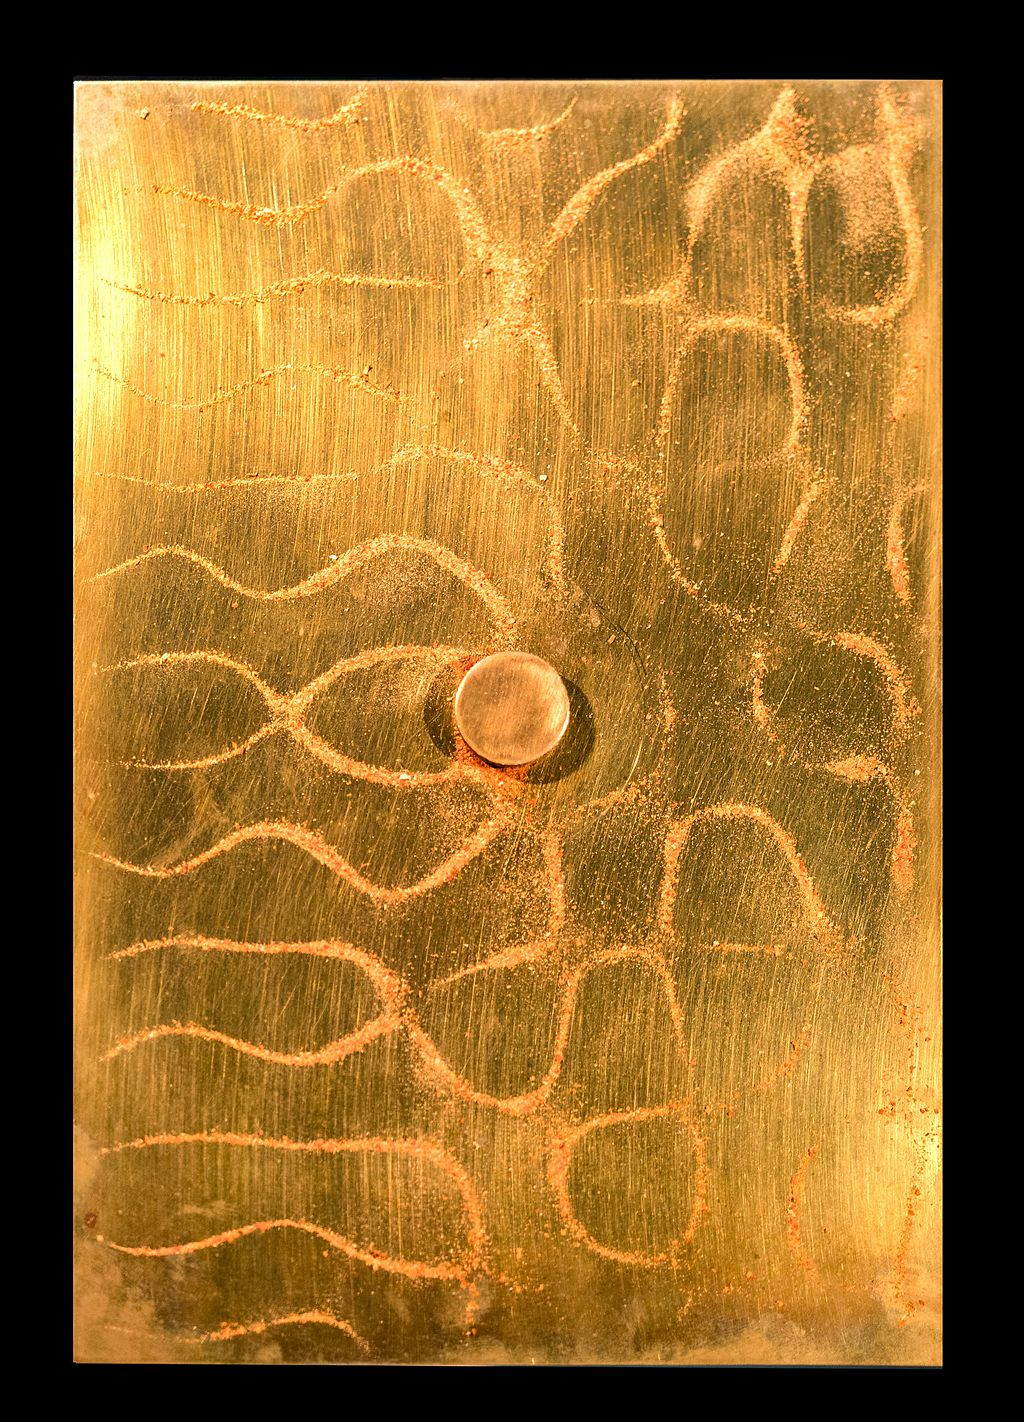
\includegraphics[height=0.3\textwidth]{Figures/chladni_plate.jpg}
		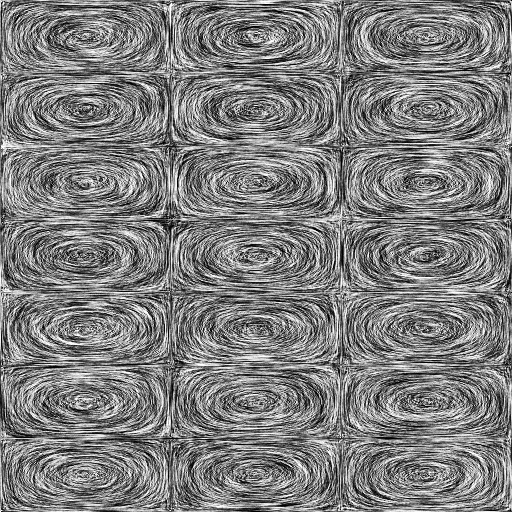
\includegraphics[height=0.3\textwidth]{Figures/LIC.jpg}
%		\vspace*{-1em}
		\caption{{\em{\bf Left:} Chladni patterns realized through a physical experiment. Source: Wikimedia Commons.} {\em{\bf Right:} Analytic 2D eigenvector of the Navier-Stokes equations using the method of de Witt et al.} \cite{deWitt:2012}.}
		\label{fig:chladni-plate}
\end{figure}

\section*{Eigenvector Preliminaries}
In order to better understand the role they play in this work, we start with a review of eigenvectors and values. The eigendecomposition of a square matrix $\boldA$ is usually written as $\boldA = \QQ \Lambda \QQ^T$. The matrix $\Lambda$ is zero except along its diagonal, and each individual entry along the diagonal is an ``eigenvalue,'' where the German {\em eigen} roughly translates to ``characteristic.'' The matrix $\QQ$ is generally not diagonal, and contains columns that are each considered an ``eigenvector'' of $\boldA$. The essential character of the matrix is captured by these vectors and values because they satisfy a specific relationship. If we place the $i$th column of $\QQ$ into a vector $\qq$, and the $i$th diagonal entry of $\Lambda$ into a scalar $\lambda$, the relation $\boldA \qq = \lambda \qq$ will always hold. The vector $\qq$ will be scaled by the value $\lambda$, but will otherwise remain unchanged.

There are many different ways to understand this relationship, but the scenario of a vibrating string offers a clean physical interpretation. One way to describe the phenomenon of vibration is as one of a fixed shape that is repeatedly scaled. When a guitar string is plucked, it visibly forms the shape of a sine wave over $(0, \pi)$. Over time, the amplitude of this shape scales up to some positive value, attenuates back to zero, and then scales down to some negative value that is symmetric with the positive one. This cyclical sequence of amplitudes in time encapsulates the visual phenomenon of vibration.

The $\boldA \qq = \lambda \qq$ relation can be understood to model exactly this behavior. If the entries of $\qq$ are set to be a sine wave over $(0, \pi)$, and the entries of the matrix $\boldA$ are set according to the correct physical principles \footnote{In this case, $\boldA$ would correspond to the wave equation; a Laplacian with Dirichlet boundary conditions.}, then multiplying by $\boldA$ will produced a scaled version of $\qq$. Repeated multiplications will produce a sequence of scaled vectors, mimicking vibration. The eigenvectors thus describe a set of characteristic vibrational shapes that a string is capable of producing. The other columns of the matrix $\QQ$ describe other shapes (``vibration modes'') that a string is capable of producing. For example, sine waves defined over $(0, 2\pi)$, $(0, 3\pi)$ and up to $(0, N \pi)$ will all make an appearance. They are less dominant from a physical perspective, which is why the $(0, \pi)$ version is the one we most visually associate with a vibrating string. This dominance is reflected in the eigenvalue analysis; the $(0, \pi)$ sine wave appears as the first vector in $\QQ$, and each successive column yields progressively less visually and sonically important shapes.

This understanding can be extended to both 2D and 3D, but some effort is needed to rearrange these higher-dimensional phenomena so that they can be packed into a 1D vector $\qq$. For example, we can cut a square 2D plate into a regular grid, and rearrange the 2D values defined over this grid into a 1D vector $\qq$. Again, a matrix $\boldA$ can be assembled according to physical principles so that its eigenvectors correspond to the characteristic vibrations of a square plate. When these eigenvectors are unfolded back into a 2D grid, their visual character is in close agreement with those found by laboratory experiments (Figure \ref{fig:chladni-plate}).

%\section*{Computational Fluid Dynamics Preliminaries}
\section*{Empirical Eigenvectors in Computational Fluid Dynamics}

The eigenvector analysis that automatically discovers Chladni patterns does not extend directly to more complex phenomena. Nevertheless, we are interested in discovering analogous patterns that arise in turbulent fluid flows. The equations for these flows are inherently non-linear, while the eigenvector approach is inherently linear, so we will instead use the method of ``empirical'' eigenvectors. In order to motivate and elucidate these techniques, we will introduce some concepts from computational fluid dynamics (CFD).

A fluid is usually defined using a velocity field, where a velocity vector is associated with each point in space. While there are many different ways to represent these fields, we take the perspective from the previous section where a bounded region of space has been diced into a set of regular squares (or, in 3D, cubes). Each cube is then assigned a corresponding velocity vector (Fig.~\ref{fig:velocity-field}), and in order to generate an animation, the vectors must then be evolved over time. There are many different equations that can be used to specify this evolution in time, but we used the well known incompressible Navier-Stokes equations for fluid flow. A detailed discussion of these equations is beyond the scope of the current work, so we will instead assume that we have divided time into a discrete number of steps, and that at each step, the vector inside each cube in our computational grid has a corresponding value. Further details on the numerical integration methods we employ can be found in the paper by Stam \cite{Stam99}.

%We begin with a brief discussion of some fundamental techniques in computational fluid dynamics (CFD). Fluid flow is typically represented by a velocity fields, which associate a velocity vector to each point in space. For computational purposes, we regularly partition space discretely into many small cells so that each cell has an associated velocity vector (Fig.~\ref{fig:velocity-field}). To create animations, the velocity fields must also evolve over time. To that end, the incompressible Navier-Stokes equations are a well-known set of differential equations which model the time evolution of fluid flow. Although a detailed discussion of these equations is beyond the scope of the current work, on a high level, assuming we have a computational approximation to these equations, this means we can subdivide time into discrete timesteps and simulate the evolution of each velocity vector in each cell as it changes from one timestep to the next. 

\begin{figure}
		\centering
		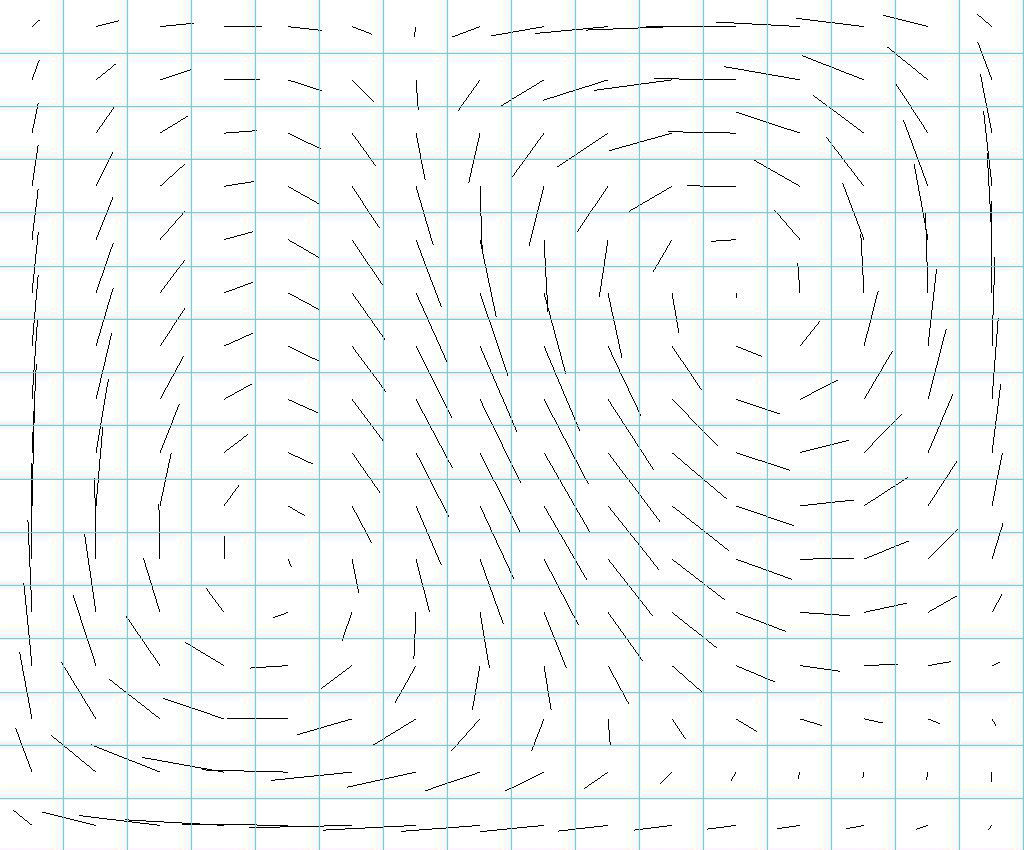
\includegraphics[height=0.3\textwidth]{Figures/velocity_field.png}
		\caption{\em A $2\textnormal{D}$ velocity field on a regular grid.}
		\label{fig:velocity-field}
\end{figure}

Unlike the classic Chladni pattern case, CFD simulations do not yield a single matrix $\boldA$ on which an eigenvalue analysis can be performed, as the non-linear operations involved generate a new, time-dependent matrix $\boldA$ at every timestep. Instead of one canonical $\boldA$ that can be said to characterize the behavior of the entire system, there are instead infinite $\boldA$s, none of which inherently take precedent over others. Fortunately, if some sort of precedence is imposed, something akin to an eigenvalue analysis can still be applied.
The method of ``empirical'' eigenvectors \cite{Ryckelynck2005}, also known as the a Proper Orthogonal Decomposition, Karhunen-Love expansion, or Hotelling transform, establishes one such criterion. Informally, given an existing simulation, we can analyze the series of matrices that arose during that simulation, and give those matrices precedence over all others. The space of infinite $\boldA$s is thus reduced to a tractable, finite size.

%\section*{Empirical Eigenvectors of a Fluid}
%In this section, we would like to discover a characteristic set of velocity fields that can be combined to generate a wide range of fluid motions. Given a particular mathematical operator, we can study its eigenvectors, or characteristic vectors. These vectors, loosely speaking, are the inputs to the operator that transform by scaling only. Eigenvectors are especially useful if we can describe arbitrary inputs to the operator as a mixture of eigenvectors, since this allows us to easily compute the outputs.

%In our work, the operator in question is the Navier-Stokes equations for fluid flow. There are several different strategies for computing the eigenvectors associated with this operator. For example, de Witt et al. \cite{deWitt:2012} computed the analytic eigenfunctions of the fluid velocity field over a simple square domain, and used them to advect (i.e.~push) a particulate through space. These eigenfunctions are composed of separable products of sines and cosines, and the results visually correspond closely to classic Chladni patterns (Fig.~\ref{fig:chladni-plate}, right).

%We are interested in generating less classical results, so we prefer the use of ``empirical'' eigenvectors~\cite{Ryckelynck2005}. This approach goes by many names, such as the Proper Orthogonal Decomposition, Karhunen-Love expansion, or Hotelling transform, but we prefer the eigenvector nomenclature because it clarifies the connection to Chladni patterns. As the name suggests, it involves computing the eigenvectors of an empirically obtained data set, which in this case is the results of a CFD simulation.

Returning to Figure \ref{fig:velocity-field}, we first perform a simulation over a regular $N \times N$ grid for $T$ timesteps. While the simulations in our actual experiments were run in 3D (Figure \ref{fig:eigs}), we will limit discussion to 2D for simplicity. Each grid cell then contains a 2D velocity vector which possesses an $x$ and $y$ component, so the entire grid contains $N \times N$ such vectors. We can thus rearrange these values so that they are packed into a 1D vector $\xx$, which has $2N^2$ entries. We can perform this repacking for each of the $T$ velocity fields from the simulation, and concatenate all of the vectors into a matrix $\boldX$ with $2N^2$ rows and $T$ columns.

Generally, $2N^2 \neq T$, so the matrix $\boldX$ will be rectangular, and an eigenvalue analysis can only be performed on square matrices. However, the singular value decomposition (SVD) can always be performed regardless of dimension, and the results possess many eigenvalue-like qualities. Instead of the eigen-decomposition $\boldA = \QQ \Lambda \QQ^T$, the SVD instead yields $\boldX = \UU \Sigma \VV^T$. Similar to the eigen-decomposition, the middle matrix $\Sigma$ is diagonal, and its entries correspond to the ``singular'' values of the matrix $\boldX$. Again, similar to the eigenvalue case, the columns of the left matrix $\UU$ form an ordered set of the most important shapes, or quasi-vibration modes, that appeared during the simulation. The matrix $\VV$ is a $T$-dimensional rotation matrix that was applied to $\boldX$ in order to arrive at $\UU$ and $\Sigma$; for our purposes, it can be discarded.

%Recall from the previous section that our simulation of velocity fields discretizes both space and time. Hence, suppose we have $N$ grid cells and $T$ timesteps. Each particular velocity field at any given timestep can be described by $N$ velocity vectors, one for each cell. In a $3\textnormal{D}$ simulation, this is a list of $3N$ numbers, which we can simply regard as a vector $\xx \in \R^{3N}$. If we assemble these vectors column-wise into a matrix, one for each timestep, we obtain a matrix $\boldX \in \R^{3N \times T}$ (Fig.~\ref{fig:matrices}, left). This construction will allow us to use matrix analysis tools on our simulation---in particular, the singular value decomposition (SVD). Roughly speaking, the SVD discovers a natural set of basis vectors that efficiently characterize the space of desired transformations determined by $\boldX$. More concretely, we obtain a factorization $\boldX = \UU \Sigma \VV^T$, where $\UU$ comprises the basis vectors of interest, $\Sigma$ comprises the associated singular values, which are scalars that determine the relative importance of each basis vector, and $\VV^T$ comprises the right singular vectors, which are discarded for our purposes.

\begin{figure}
		\centering
		%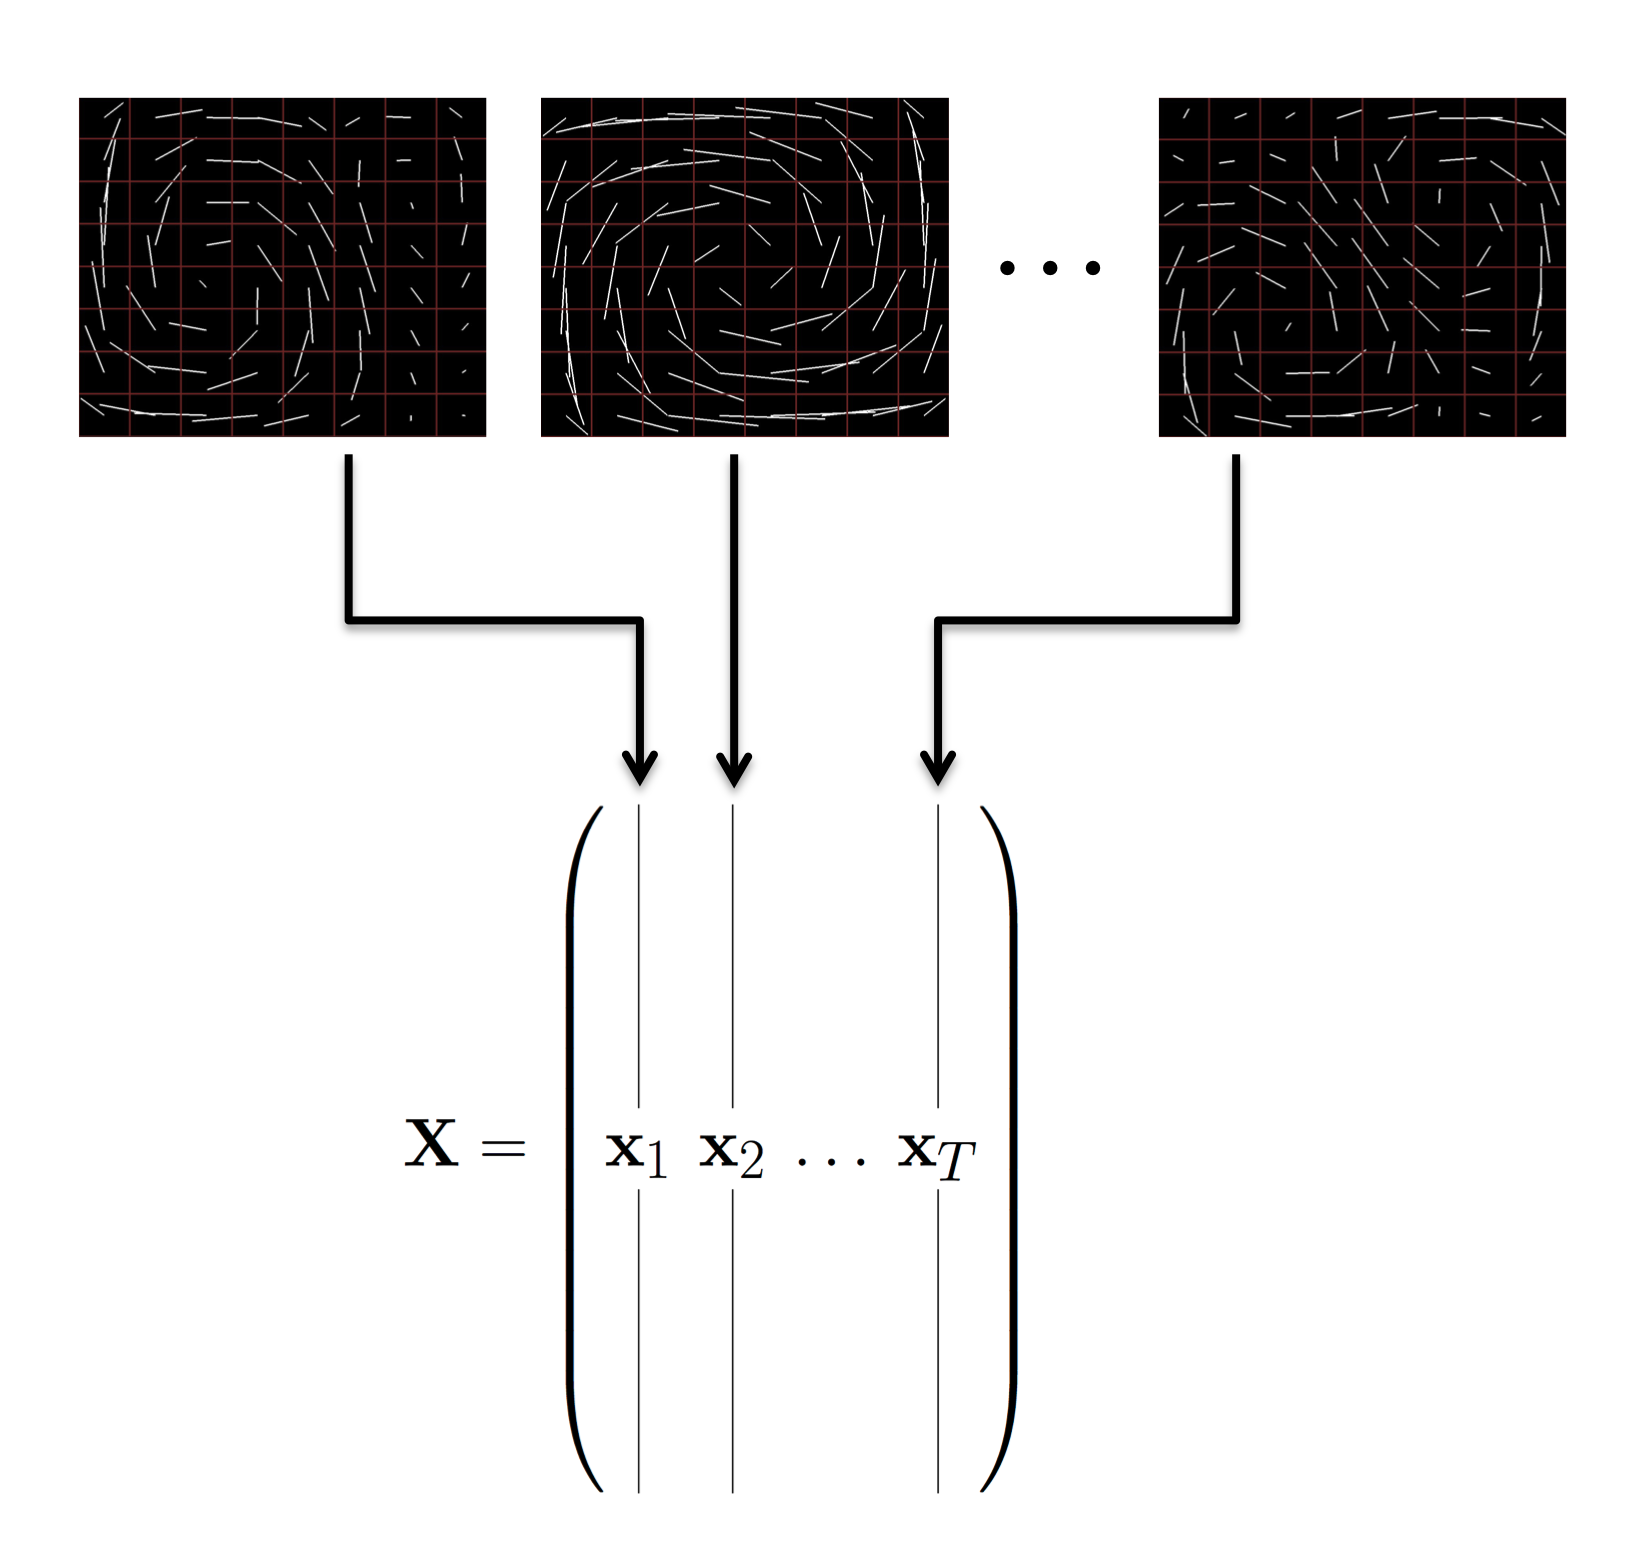
\includegraphics[height=0.45\textwidth]{Figures/assembly_matrix.png}
		%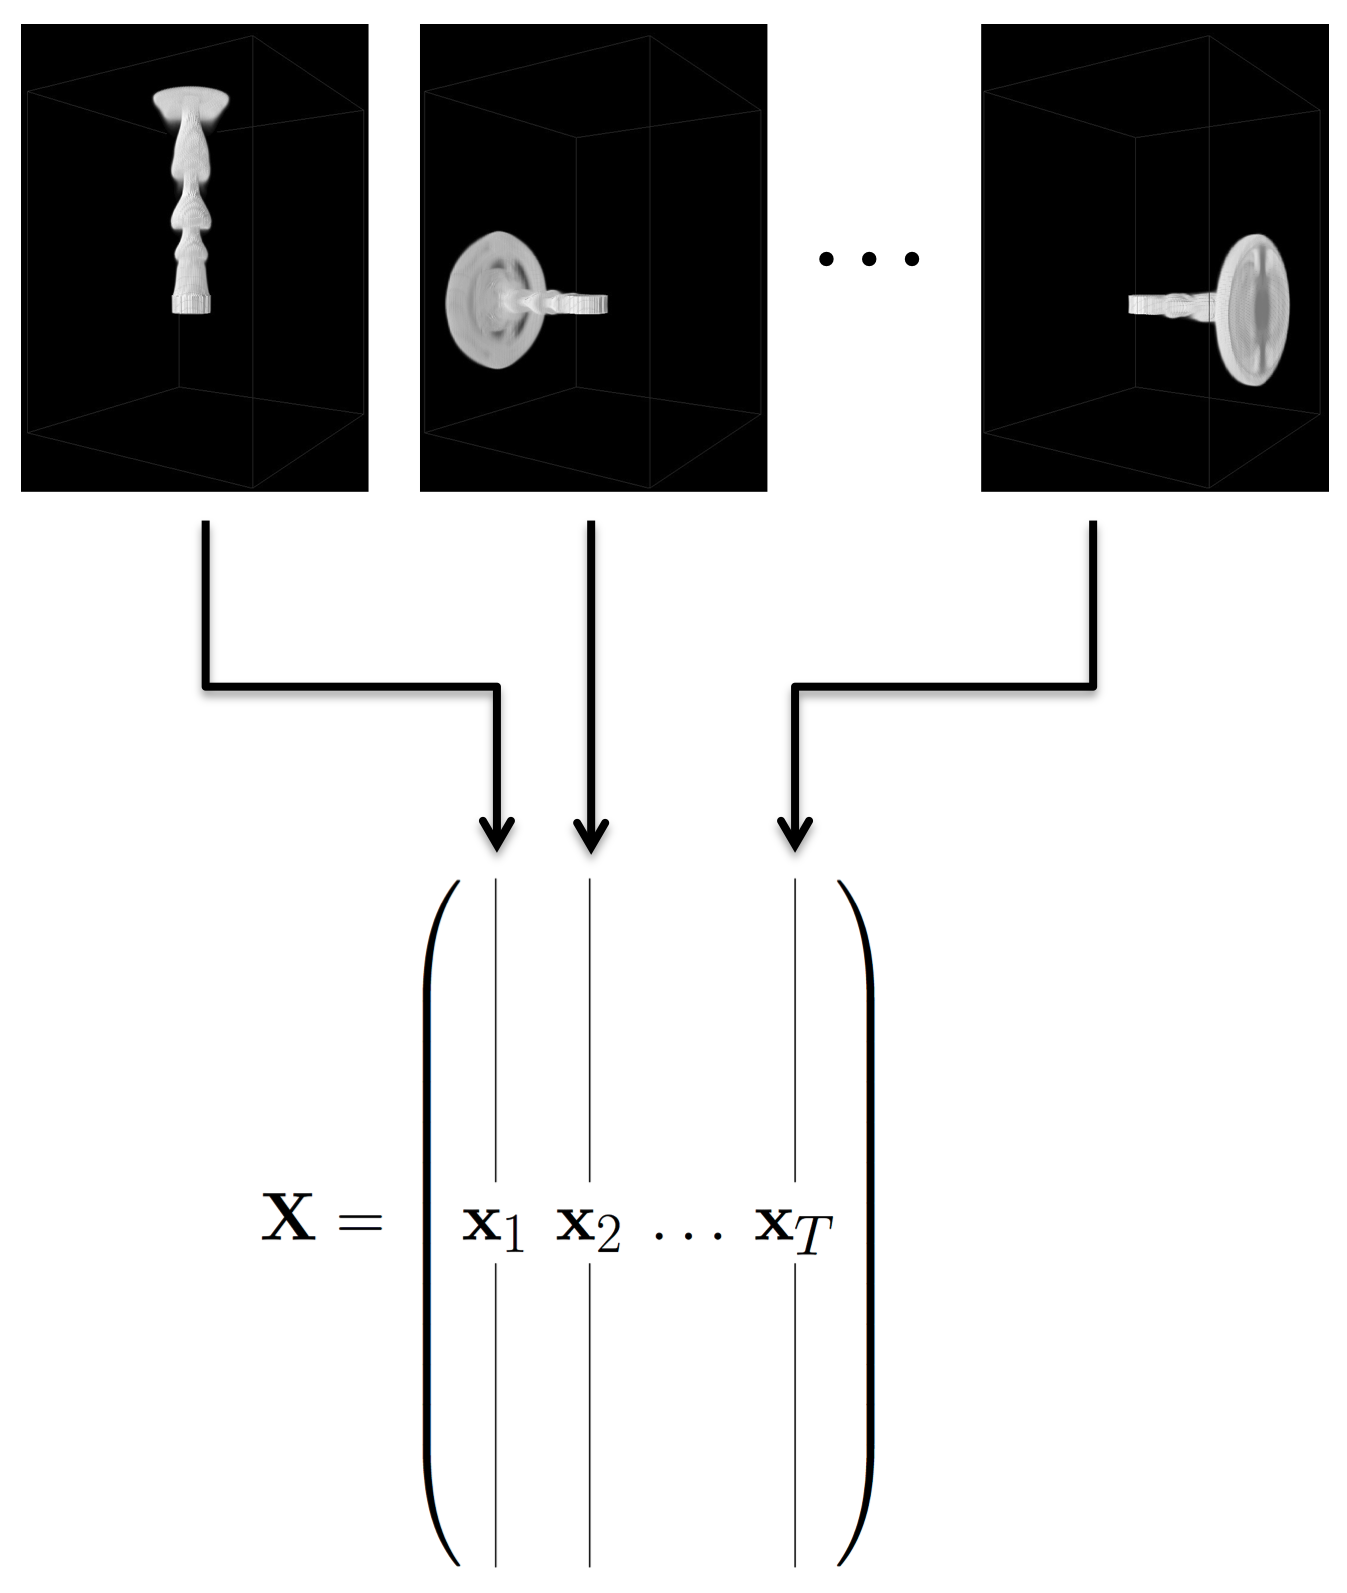
\includegraphics[height=0.45\textwidth]{Figures/plume_training.png}
		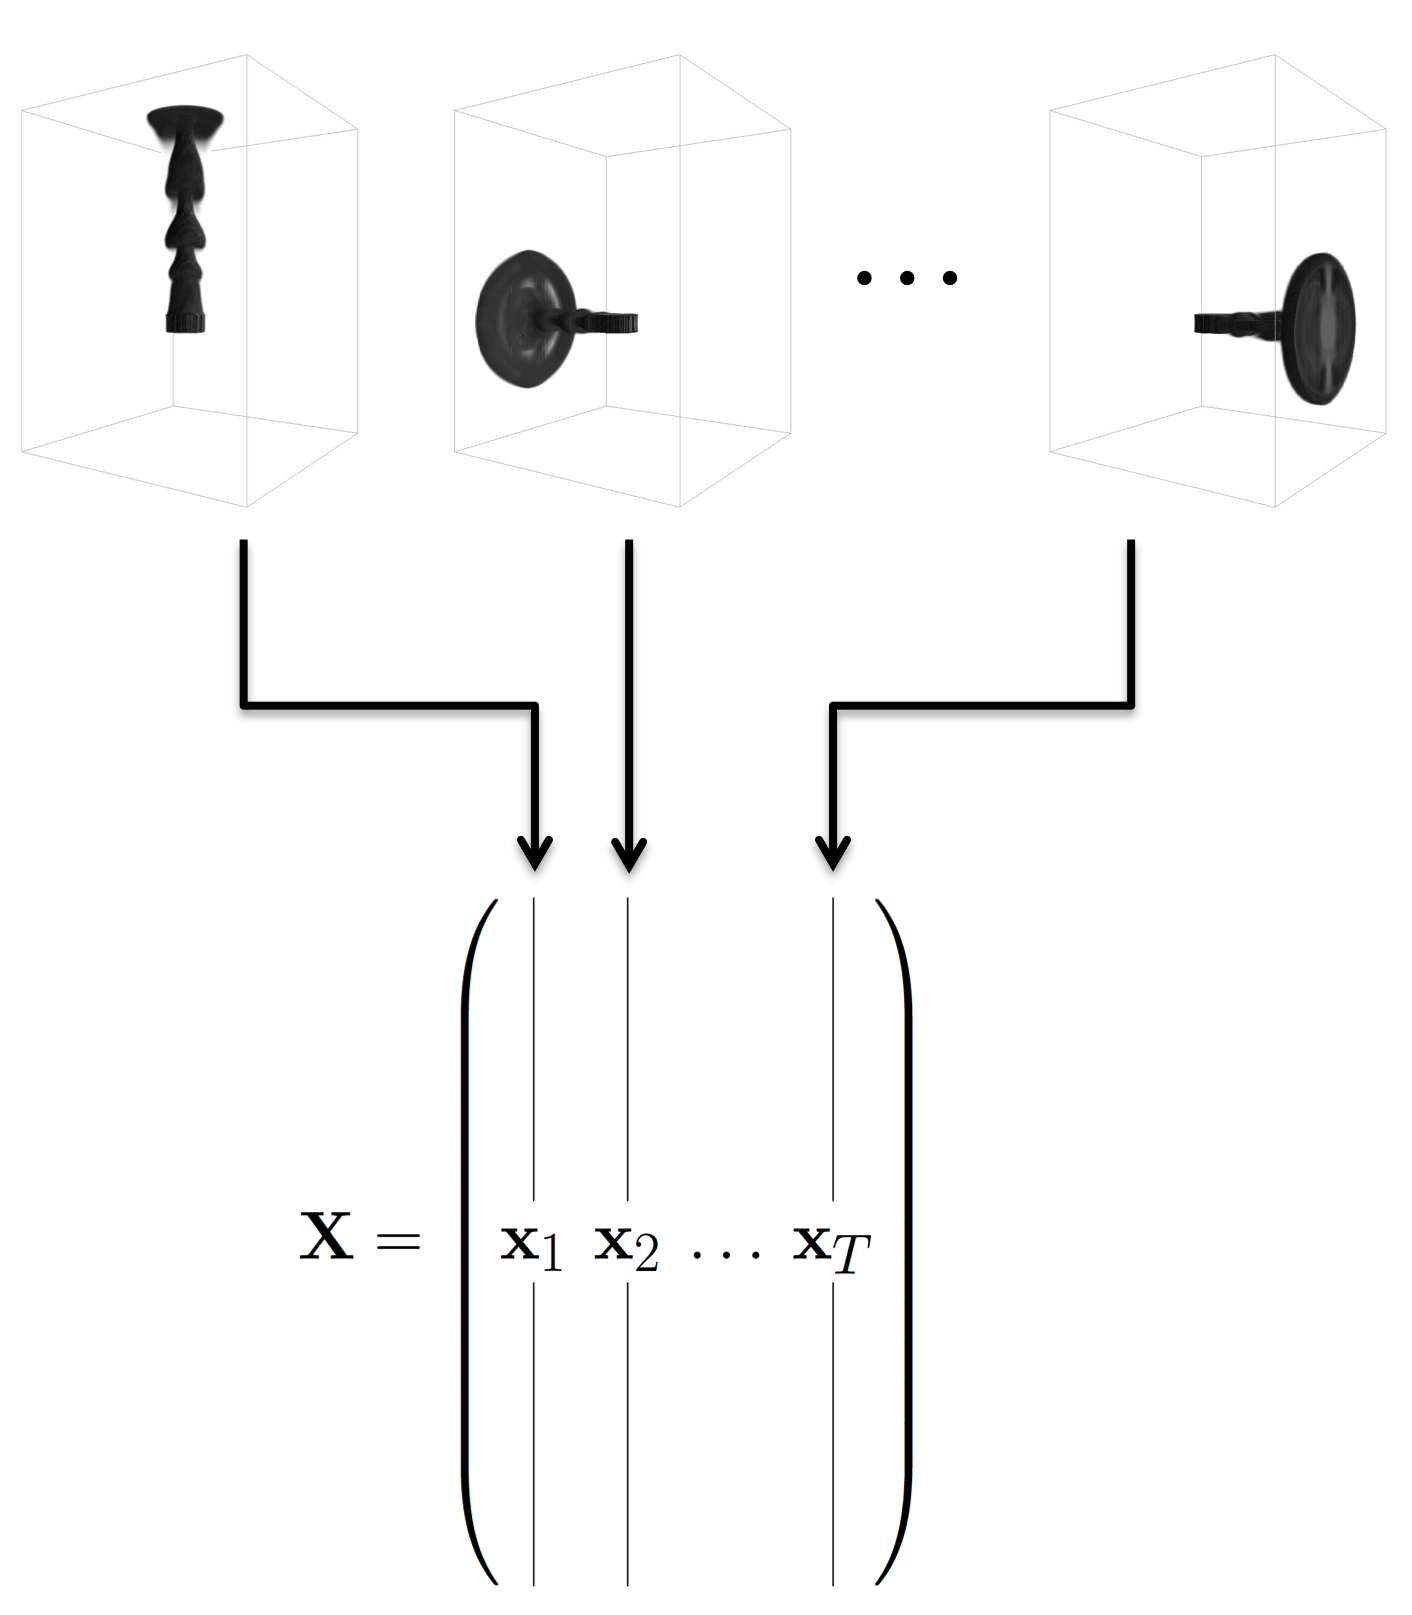
\includegraphics[height=0.45\textwidth]{Figures/plume_inverted_training.png}
		%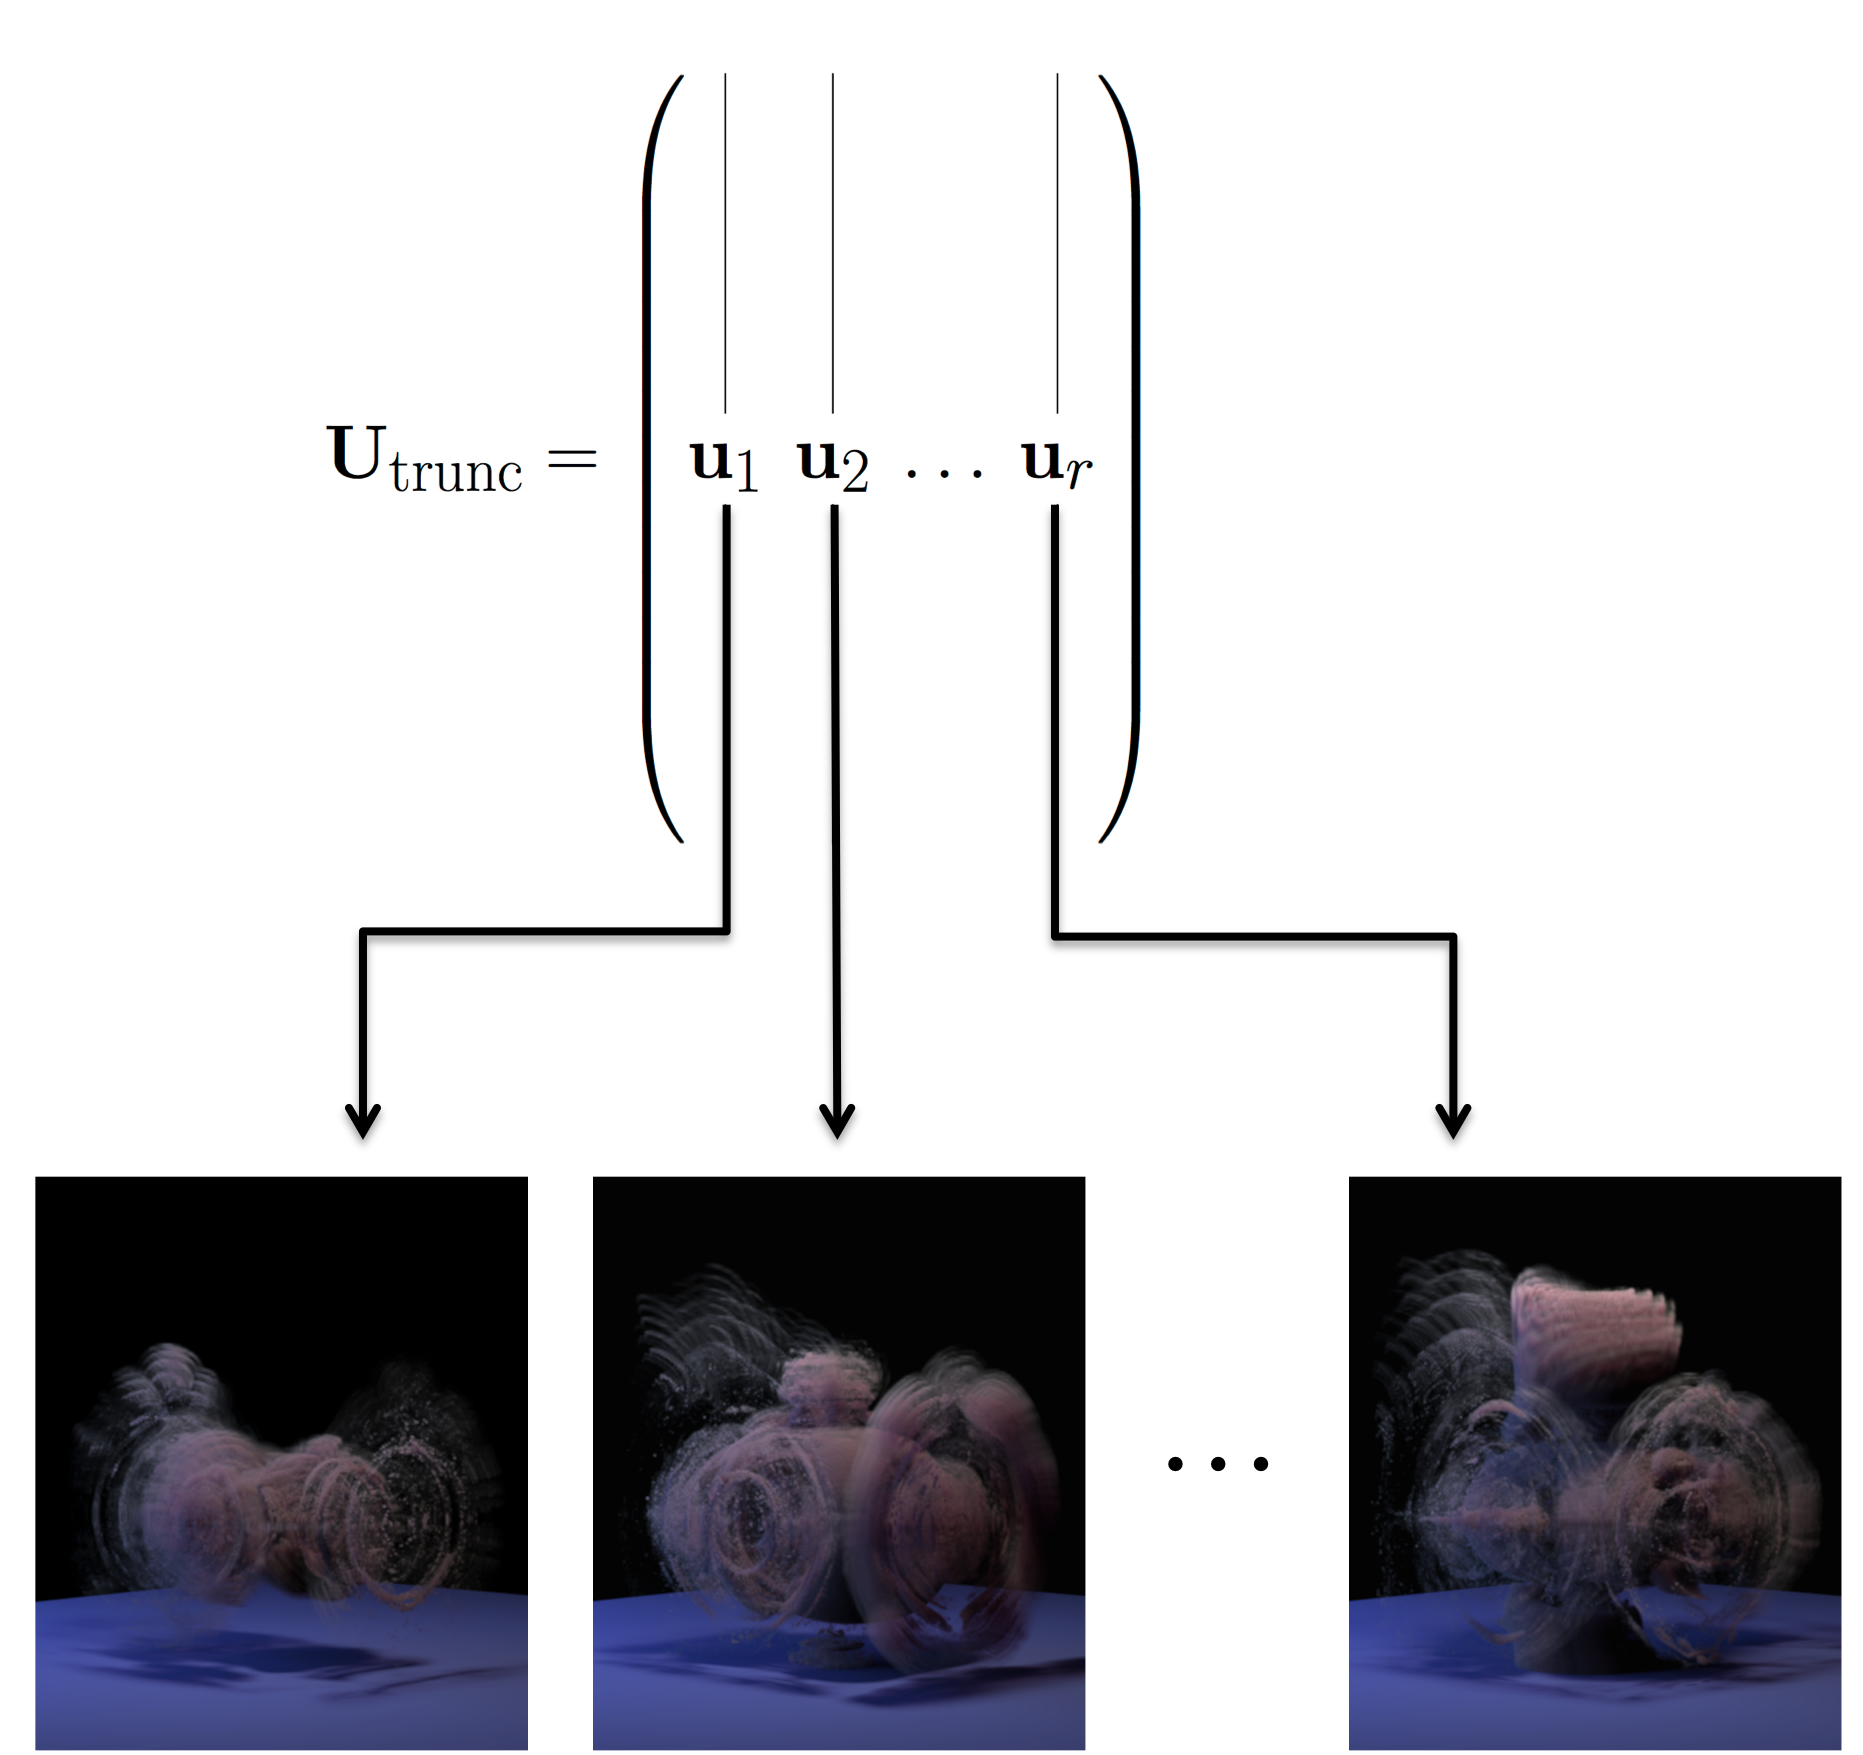
\includegraphics[height=0.45\textwidth]{Figures/U_trunc.png}
		%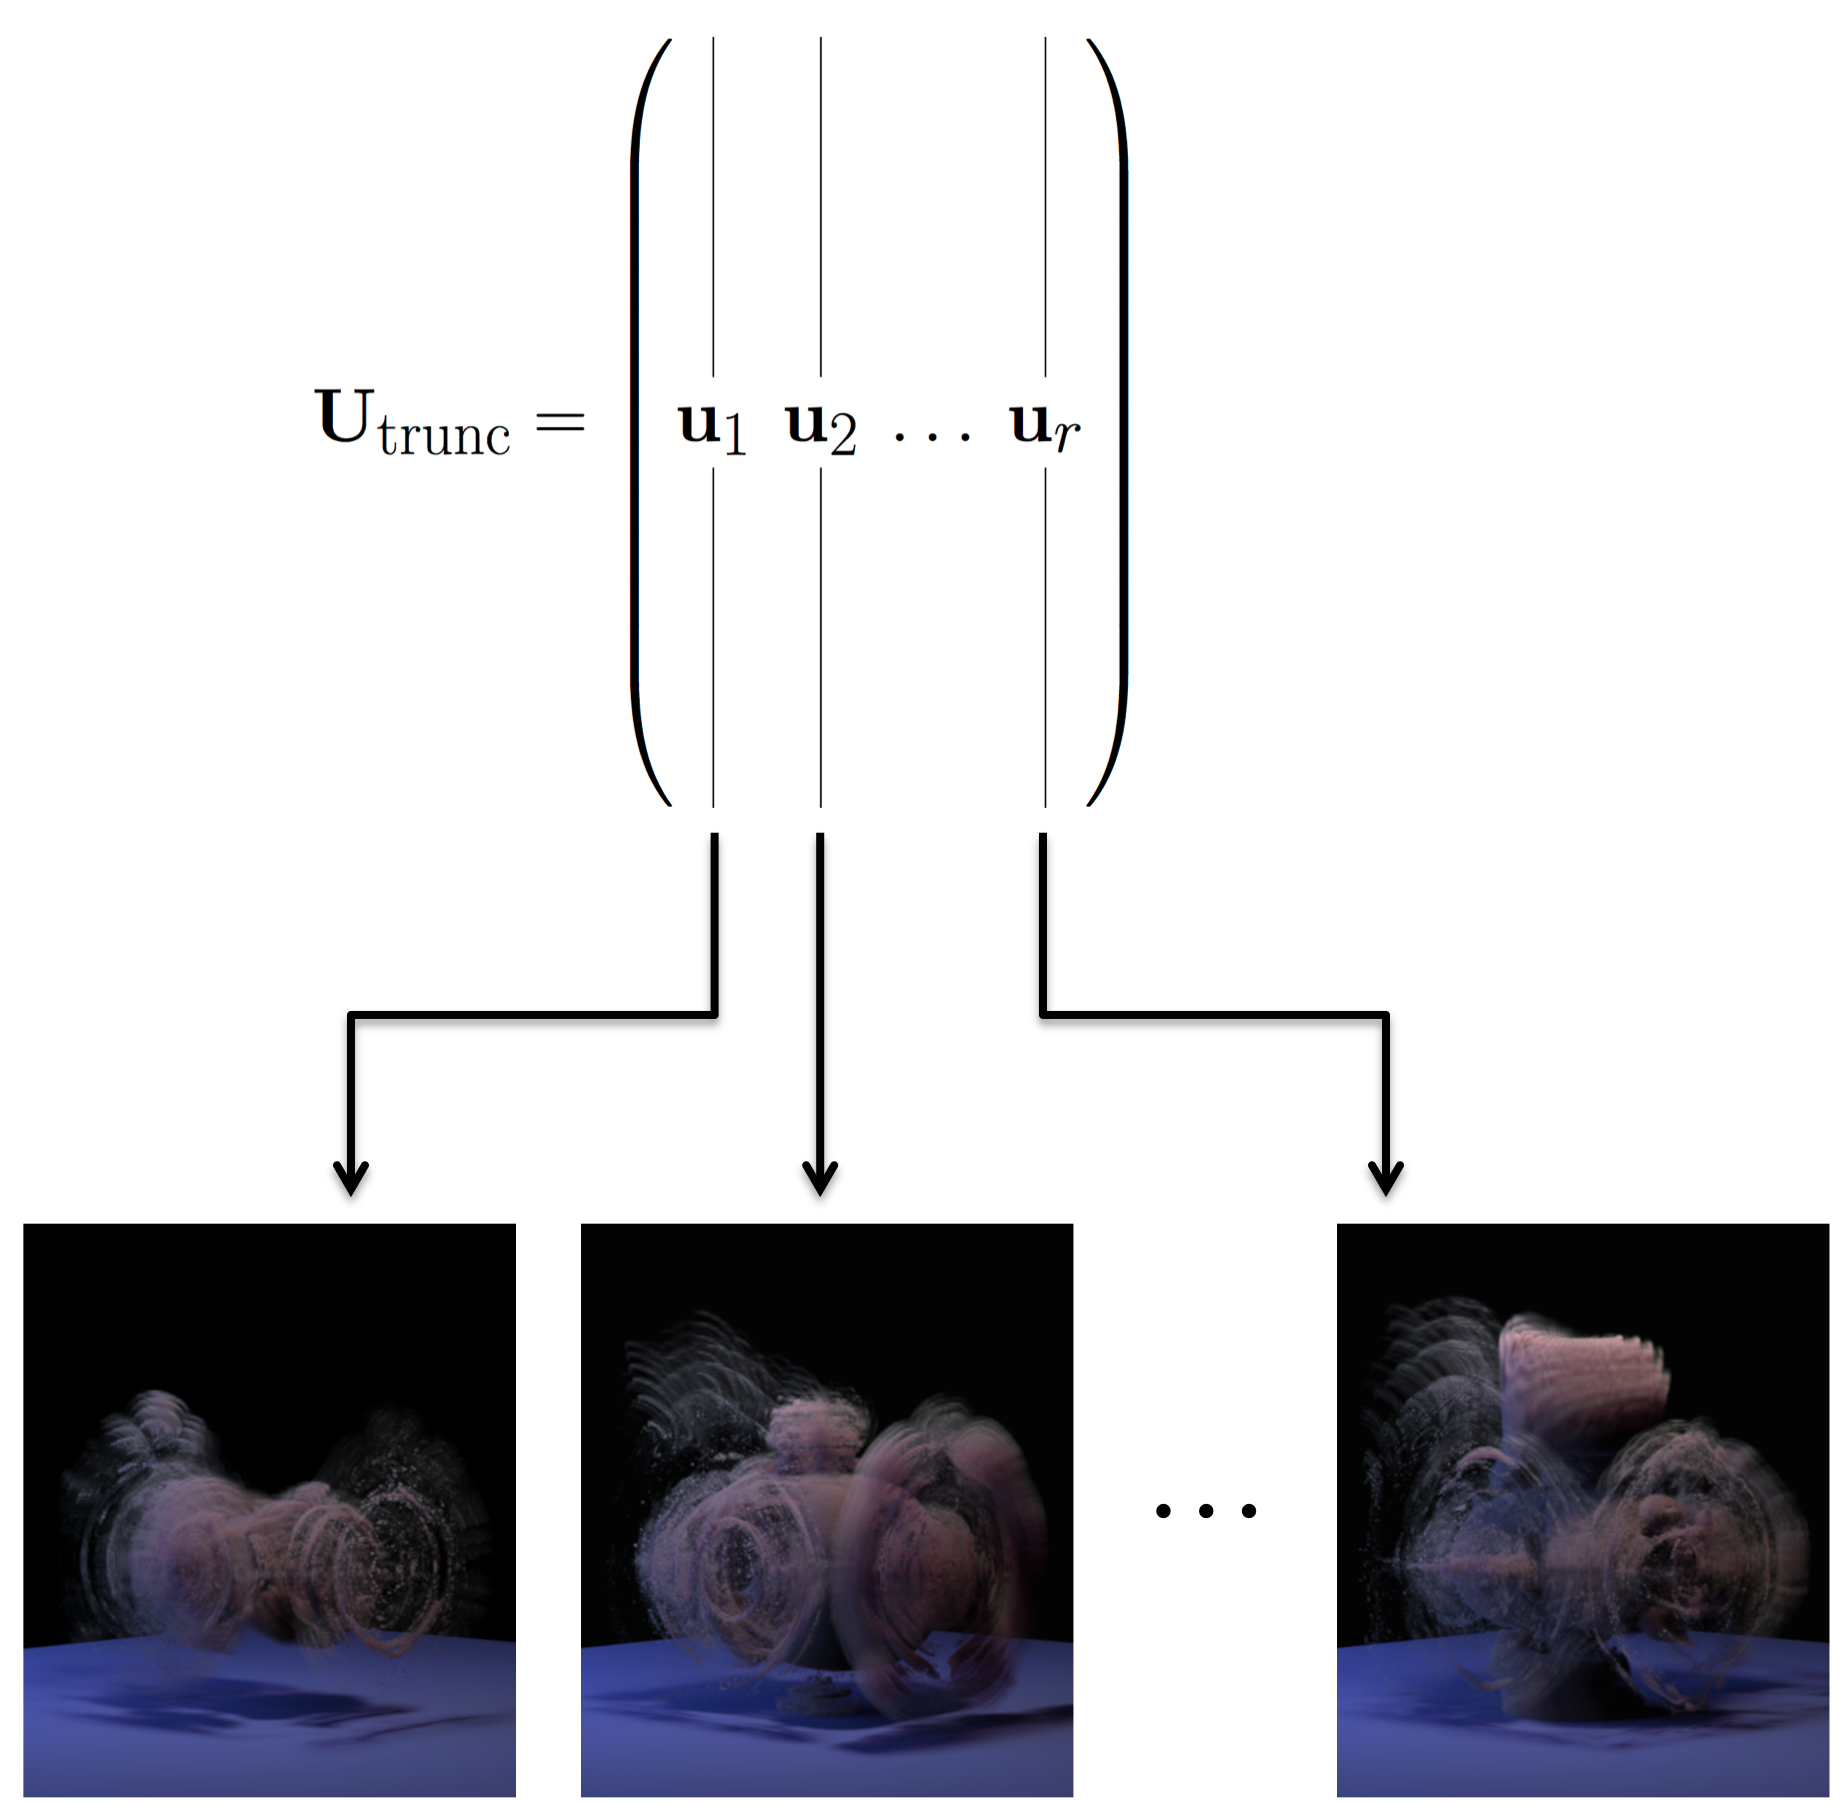
\includegraphics[height=0.45\textwidth]{Figures/U_trunc_alt.png}
		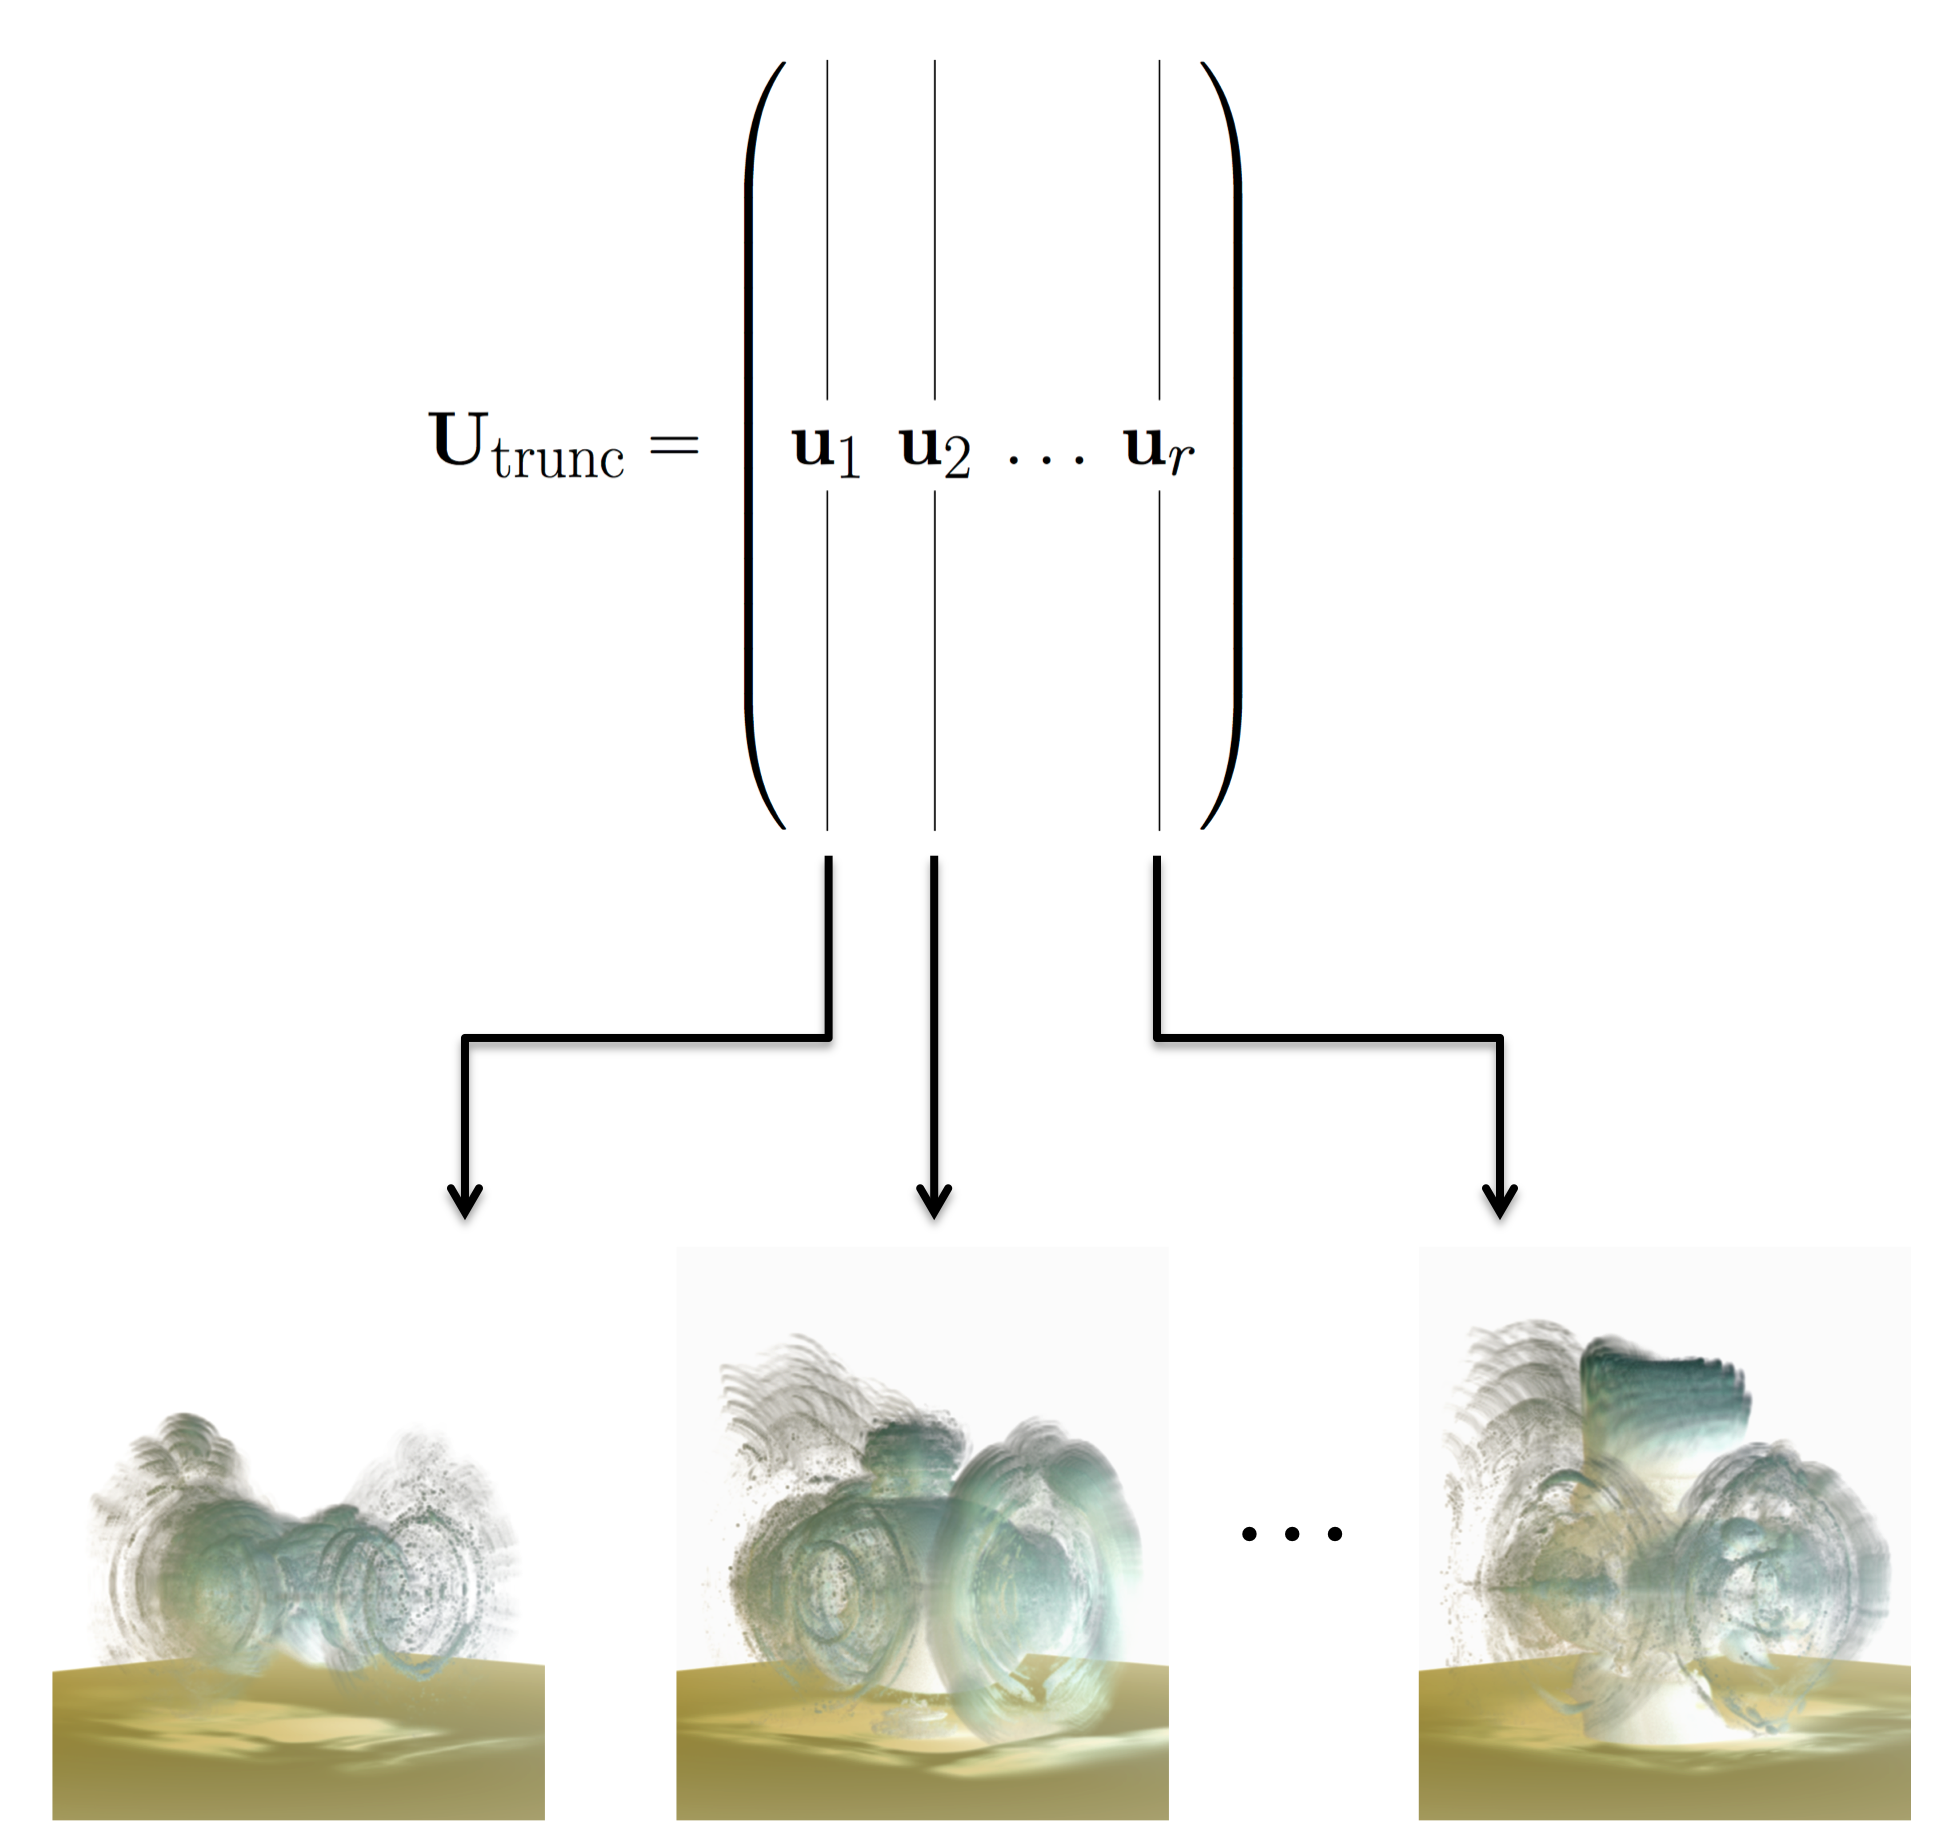
\includegraphics[height=0.45\textwidth]{Figures/U_trunc_invert.png}
		%		\vspace*{-1em}
		\caption{{\em{\bf Left:} Assembling the velocity fields column-wise into a matrix $\boldX$. We use simulations of a plume moving toward each face of its bounding box.}\\{\em{\bf Right:} Obtaining the empirical eigenvectors after the singular value decomposition is performed on $\boldX$, yielding $\truncU$. Here, $r<T$ is the number of eigenvectors we retain after truncation.}}
		\label{fig:matrices}
\end{figure}
	
%In our situation, the columns of $\UU$ are linearly independent and sorted by how well they characterize the data in $\boldX$. These columns comprise our empirical eigenvectors. Since the data in $\boldX$ is a series of fluid velocity fields, these empirical eigenvectors are the characteristic fluid velocity fields we sought which can be mixed together to describe arbitrary fluid flow. The $\Sigma$ matrix is a diagonal matrix of singular values that quantify the strength of each vector's characterization. In the special case of linear modal analysis, these values correspond directly to audio frequencies, but in the general case of arbitrary CFD simulations that we are considering, this correspondence is no longer direct. However, we will later take the occasional existence of this relationship as a launching point for our own sonification strategy. For reasons of computational space, we are only interested in the $r$ most important eigenvectors; thus, we usually truncate $\UU$ to its first $r$ columns, yielding $\truncU \in \R^{3N \times r}$ (Fig.~\ref{fig:matrices}, right).

%\todo{ADJ: This next paragraph about subspaces seems pretty dense from their perspective, but I'm not sure how to introduce it more gently.}

%The columns of $\truncU$ span an $r$-dimensional subspace $\R^r$ inside of $\R^{3N}$, and $\truncU$ itself defines a projection operator from $\R^{3N}$ to $\R^r$. For this reason, these techniques are sometimes called subspace techniques, and vectors that live in this space are called ``subspace'' coordinates, or ``subspace'' vectors. Given the $t$th velocity field from the original CFD simulation $\xx_t \in \R^{3N}$, we can compute a much smaller, subspace approximation of $\xx_t$ by computing $\truncU^T \xx_t = \qq_t \in \R^r$. The fact that subspace coordinates can be constructed in this manner has attracted significant interest in the engineering community because it is then often possible to run simulations, even those using the full Navier-Stokes equations, very quickly within this coordinate system \cite{Kim2013}.

We are interested in the representation formed by $\UU$ and $\Sigma$ for two reasons. First, these two quantities comprise a quasi-frequency spectrum. The shapes that are encoded in each column of $\UU$ are roughly analogous to the sine waves from the string case. If we take a single step from the original fluid simulation, $\xx_t$, and apply the transformation $\UU^T\xx_t = \qq_t$, then we can perform a quasi-Fourier transform that translates $\xx_t$ into a quasi-frequency domain. It then becomes straightforward to start interpreting the entries of $\qq_t$ as the amplitudes in some auditory representation. Second, an inverse-quasi-Fourier transform has also been defined. Given some arbitrary audio signal $\qq_*$, we can convert back to a spatial shape by performing the operation $\UU \qq_* = \xx_*$. Given some sound unfolding over time, we can then generate a sequence of velocity fields that drive a fluid's motion.

\todo{TK: I removed all mention of the SVD truncation here. It occurred to me that it's not actually necessary to include this. The motivation that some quasi-audio mapping comes out of the whole process can be conveyed without this}

Finally, empirical eigenvectors are a topic of interest in engineering because running simulations in this quasi-frequency-domain can have certain computational advantages. These are often referred to as ``subspace'' simulations. In this work, we will use the simulator described in Kim and Delaney \cite{Kim2013}, and refer the reader to that reference for further details.

%First, it is straightforward to interpret the entries in each $\qq_t$ as the amplitudes in a quasi-frequency spectrum. Therefore, they are a convenient starting point for constructing an auditory representation of fluid motion. Second, the projection can be reversed, or ``lifted.'' Given an arbitrary sound $\qq_*$ that was constructed in the quasi-frequency spectrum, we can unambiguously translate that sound into a fluid motion by ``lifting'' the vector back to the $\R^{3N}$ space. This is accomplished by computing $\truncU \qq_* = \xx_*\in \R^{3N}$, which yields a velocity field that can then be used to drive a fluid's motion.

%%%%%%%%%%%%%%%%%%%%%%%%%%%%%%%%%%%%%%%%%%%
\section*{Visualization}

One of the challenges when using empirical eigenvectors is the construction of an interesting set of eigenvectors. For example, if a set of smooth, featureless laminar flows are input into the SVD, there is no reason to believe that the shapes (a.k.a modes) encoded by the resulting eigenvectors will be visually interseting. In order to ensure that a rich set of eigenvectors are produced, we ran six separate CFD simulations using a standard fluid simulator \cite{Stam99}, where a turbulent plume of smoke was aimed at each face of a rectangular simulation domain. All of the simulation data was then concatenated into a matrix $\boldX$. To reveal the shape of the modes, we then ran a series of simulations with each of the modes sequentially isolated. A ``delta'' vector $\qq_d$, similar to an impulse response, was generated at each timestep where the $d$th entry is set to 1 and the rest of the vector was set to zero. A sequence of these results can be seen in Figure \ref{fig:eigs}.

%%%%%%%%%%%%%%%%%%%%%%%%%%%%%%%%%%%%%%%%%%%
% ADJ: These are the more direct analogy to the Chladni figures.
\begin{figure*}
	\centering
	%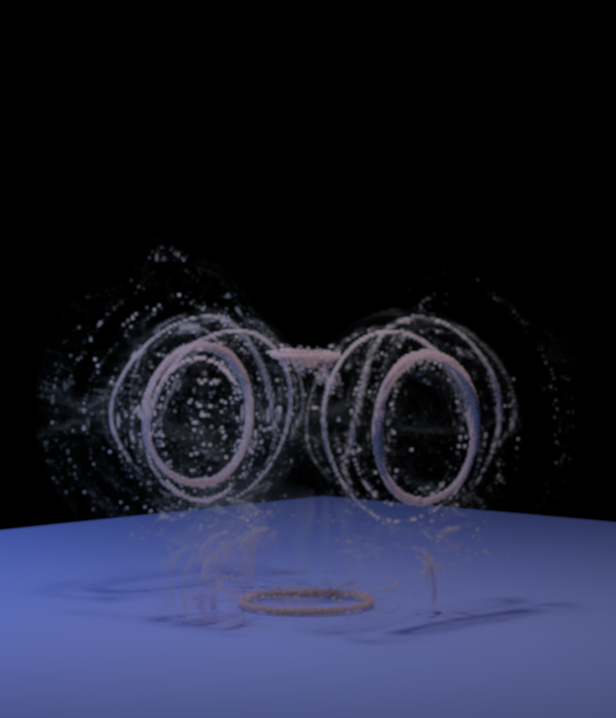
\includegraphics[width=0.24\textwidth]{Figures/modes/plume0000.png}
	%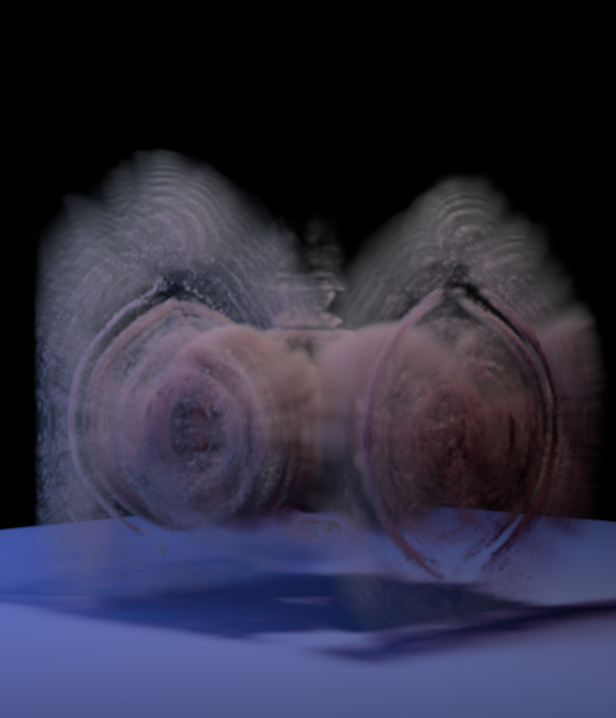
\includegraphics[width=0.24\textwidth]{Figures/modes/plume0001.png}	
	%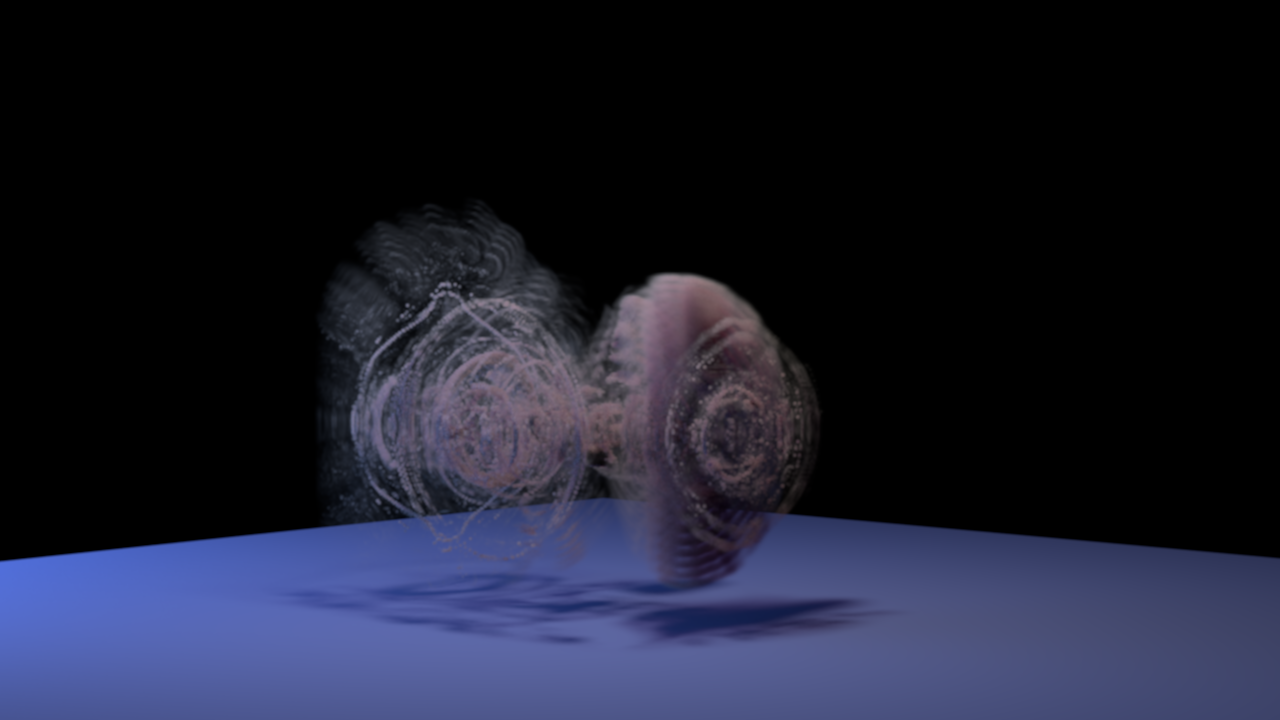
\includegraphics[width=0.24\textwidth]{Figures/modes/plume0002.png}
	%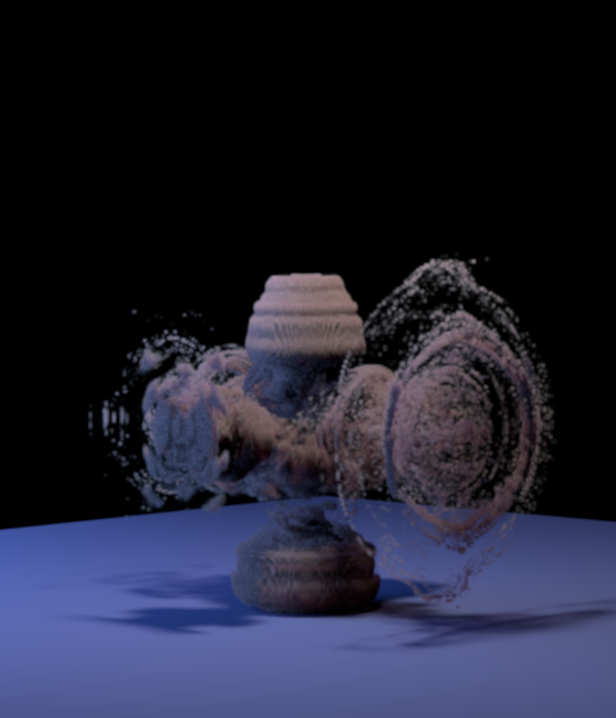
\includegraphics[width=0.24\textwidth]{Figures/modes/plume0003.png}
	%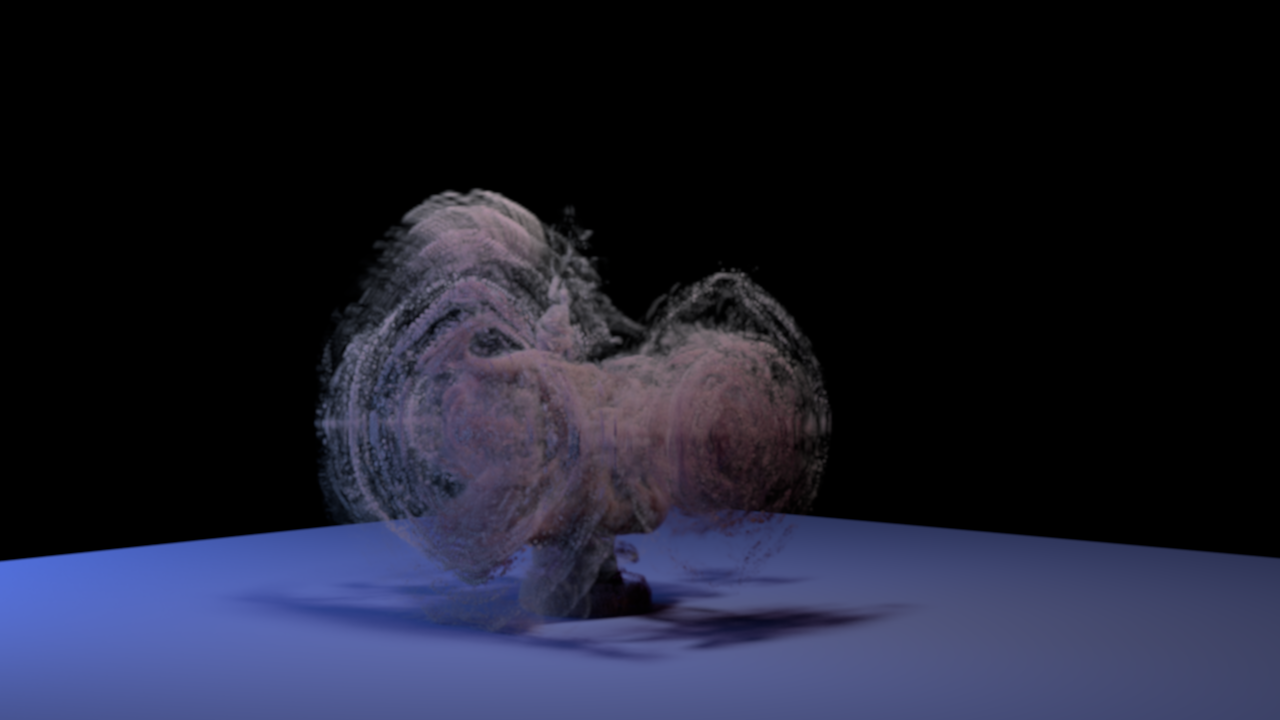
\includegraphics[width=0.24\textwidth]{Figures/modes/plume0004.png}
	%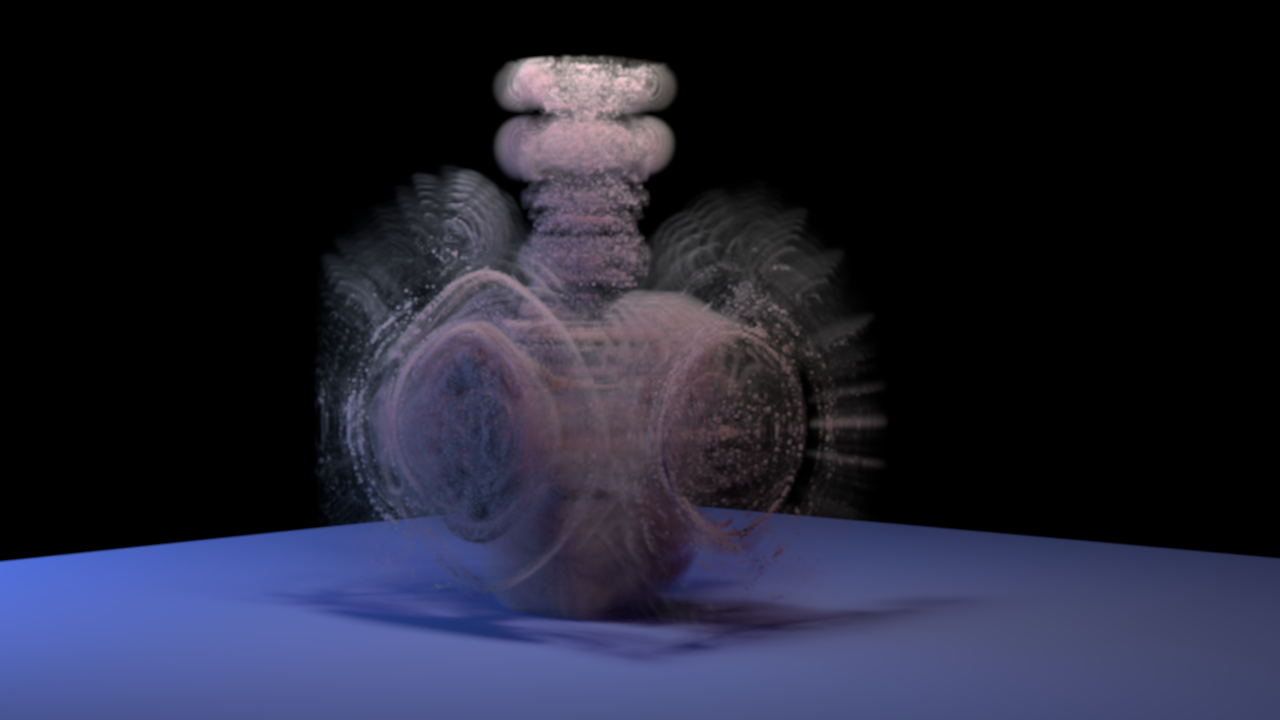
\includegraphics[width=0.24\textwidth]{Figures/modes/plume0005.png}
	%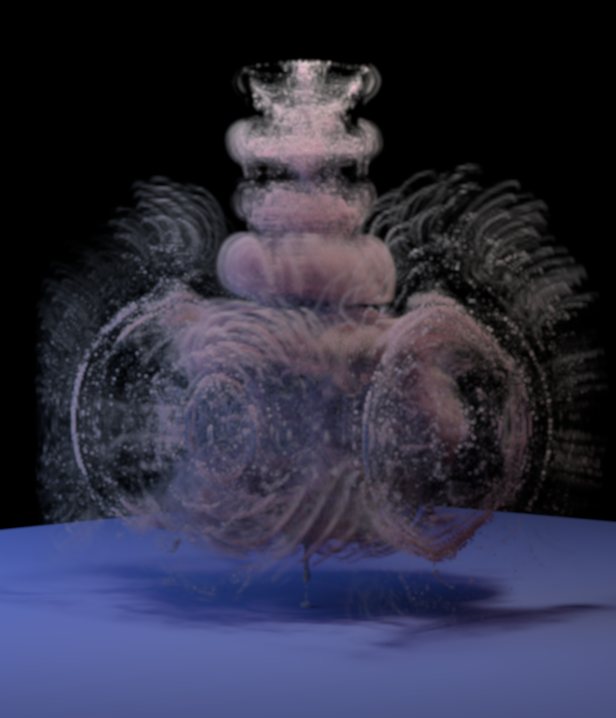
\includegraphics[width=0.24\textwidth]{Figures/modes/plume0006.png}
	%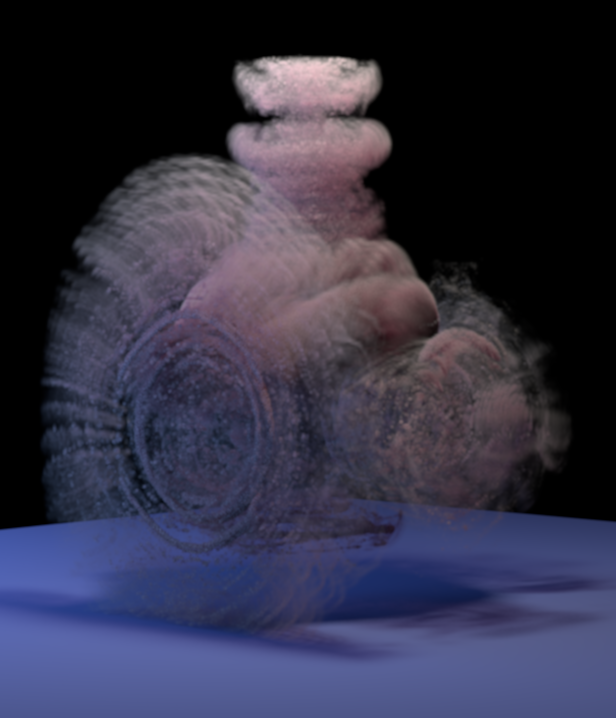
\includegraphics[width=0.24\textwidth]{Figures/modes/plume0007.png}
	%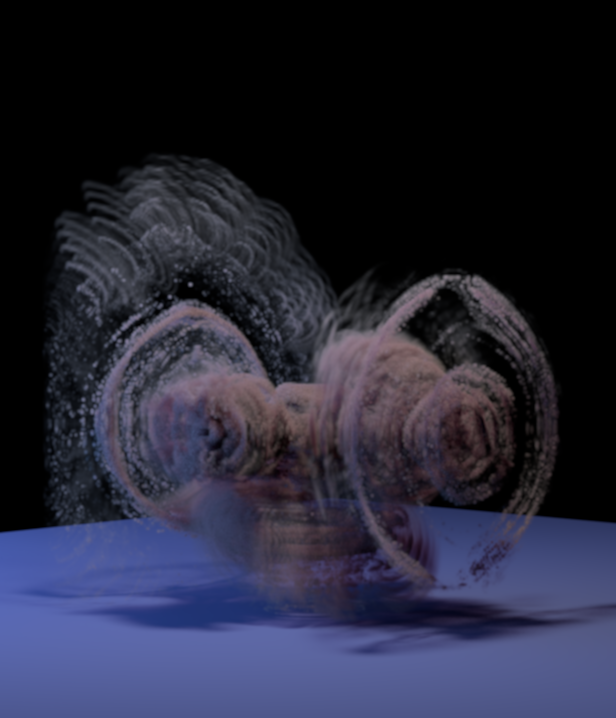
\includegraphics[width=0.24\textwidth]{Figures/modes/plume0008.png}
	%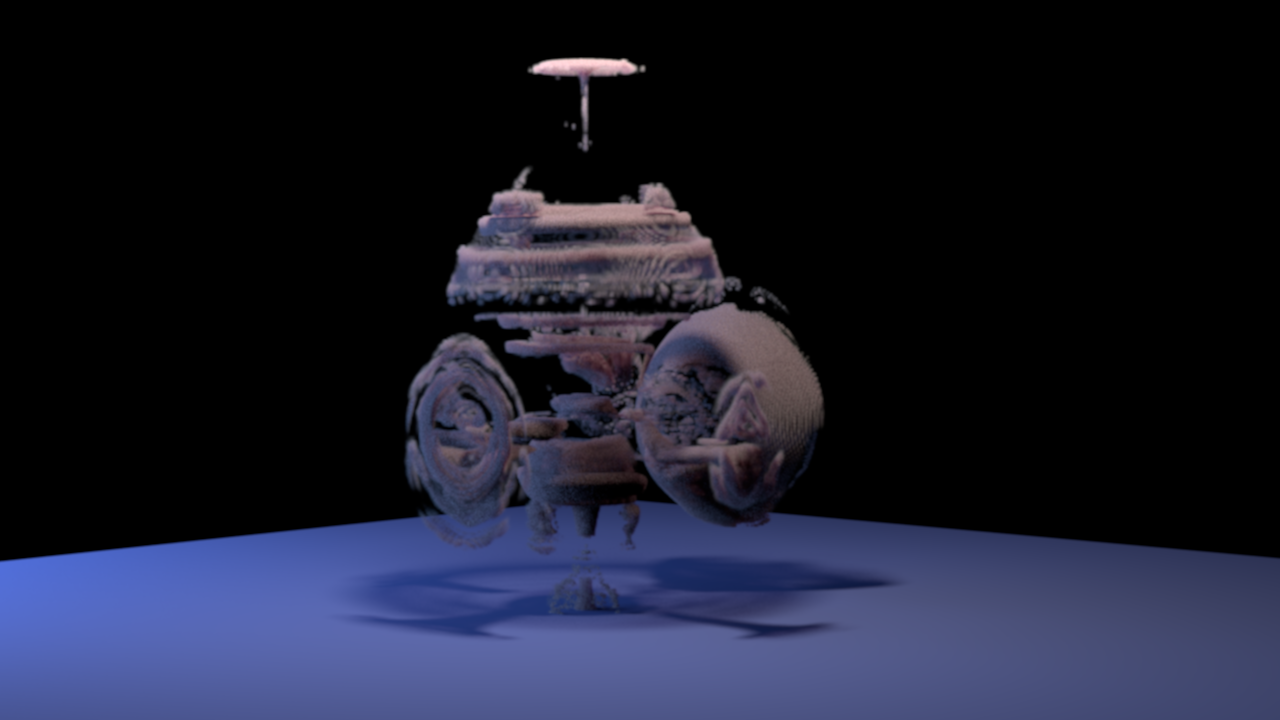
\includegraphics[width=0.24\textwidth]{Figures/modes/plume0009.png}
	%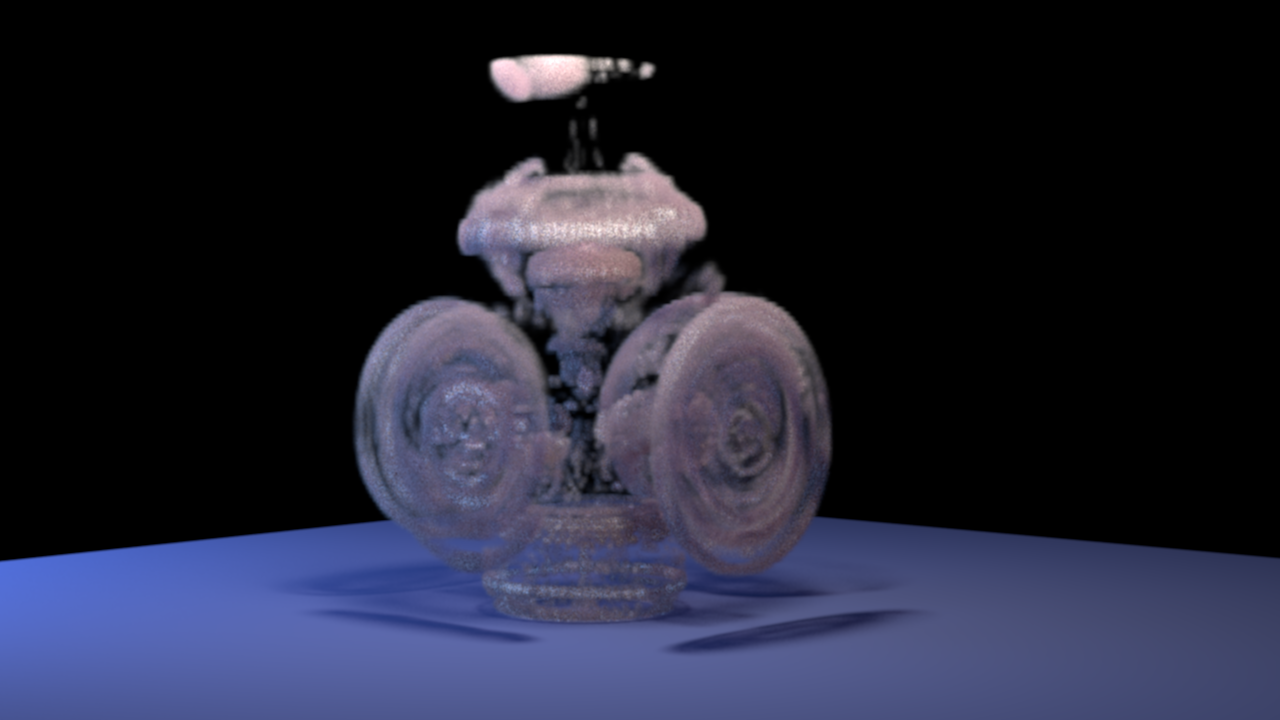
\includegraphics[width=0.24\textwidth]{Figures/modes/plume0010.png}
	%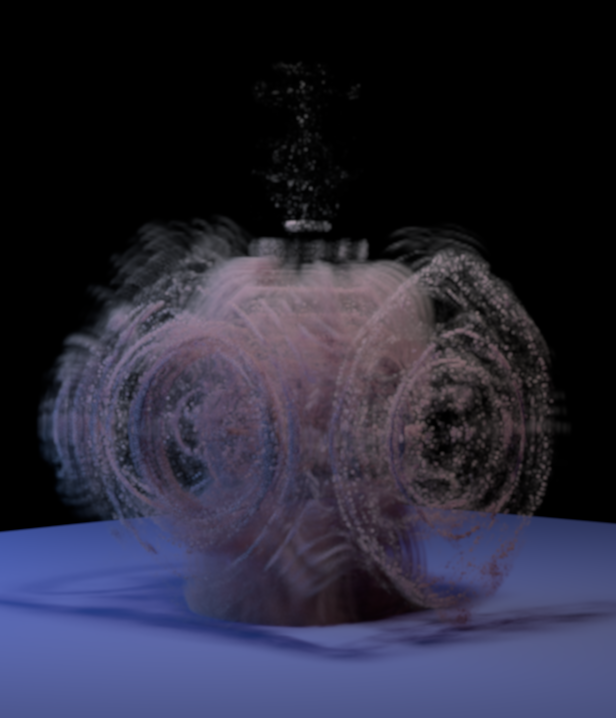
\includegraphics[width=0.24\textwidth]{Figures/modes/plume0011.png}
	%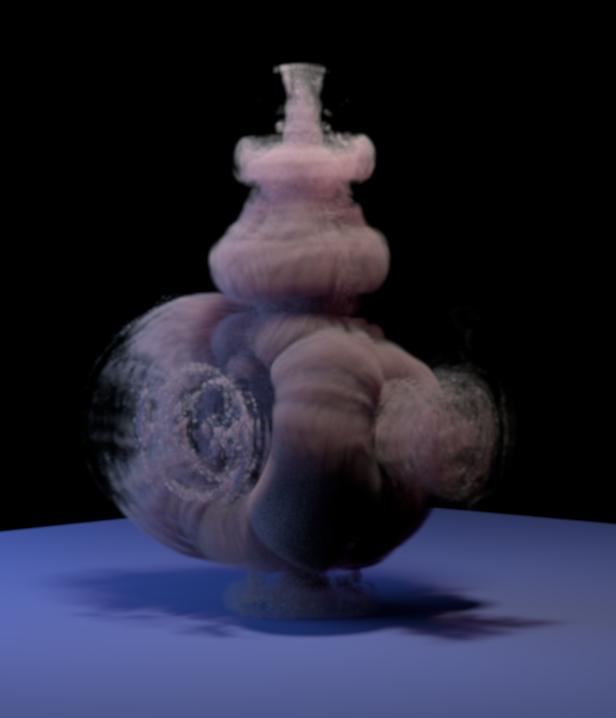
\includegraphics[width=0.24\textwidth]{Figures/modes/plume0012.png}
	%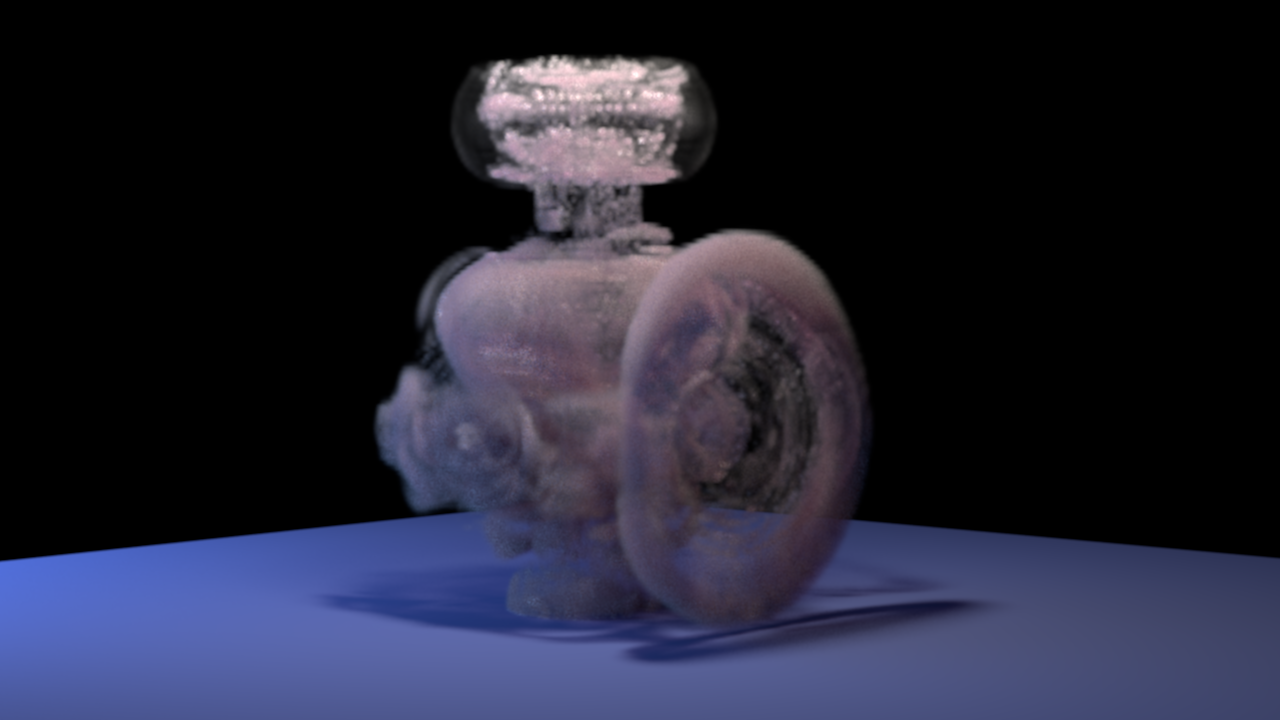
\includegraphics[width=0.24\textwidth]{Figures/modes/plume0013.png}
	%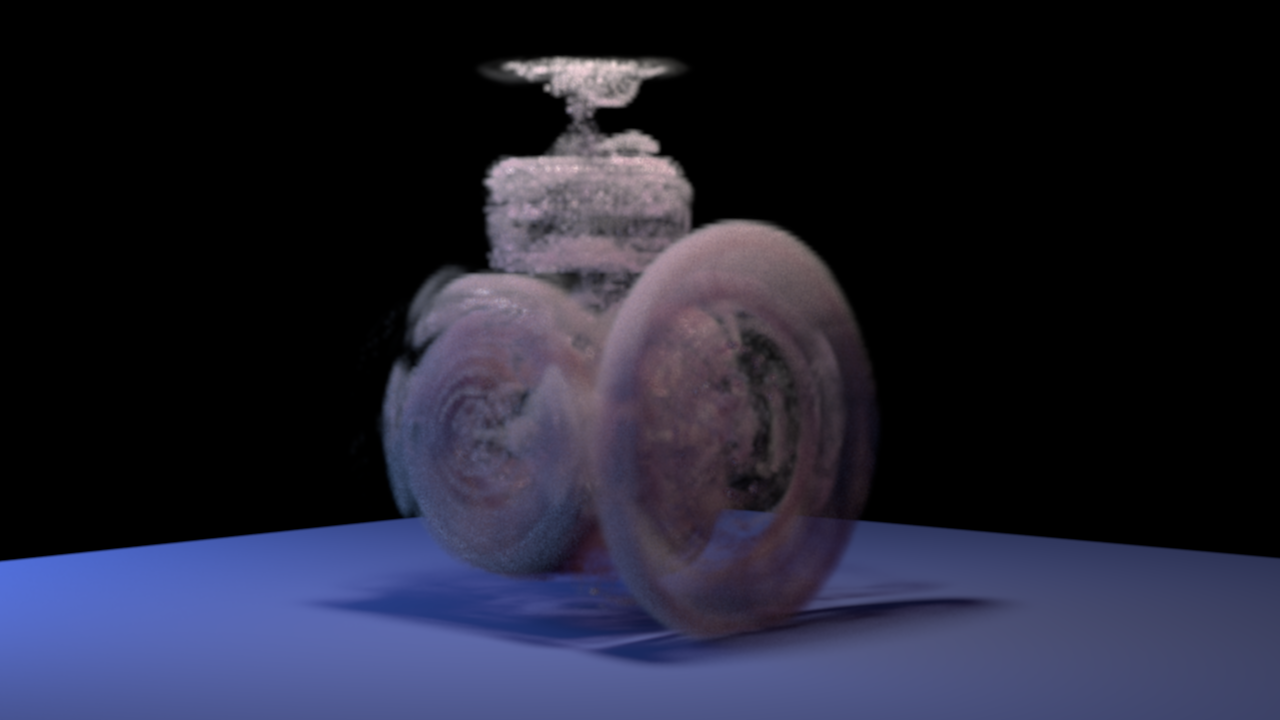
\includegraphics[width=0.24\textwidth]{Figures/modes/plume0014.png}
	%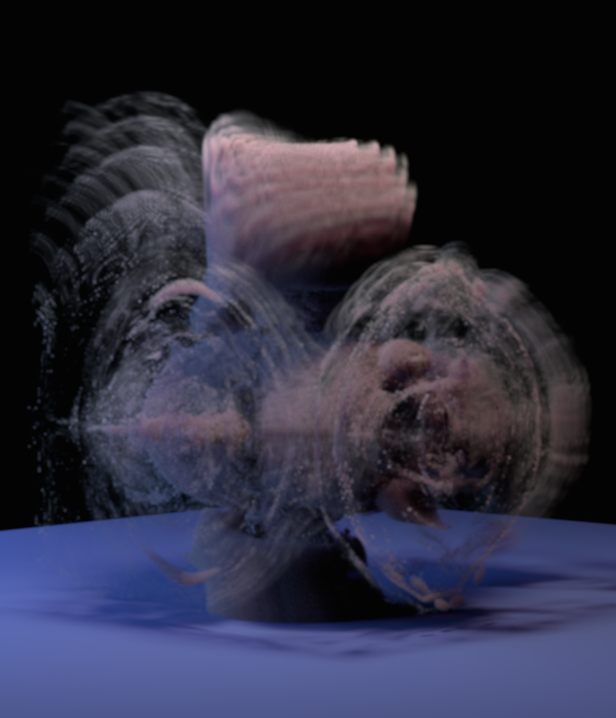
\includegraphics[width=0.24\textwidth]{Figures/modes/plume0015.png}
	%\includegraphics[width=\textwidth]{Figures/modes/montage_inverted.png}
	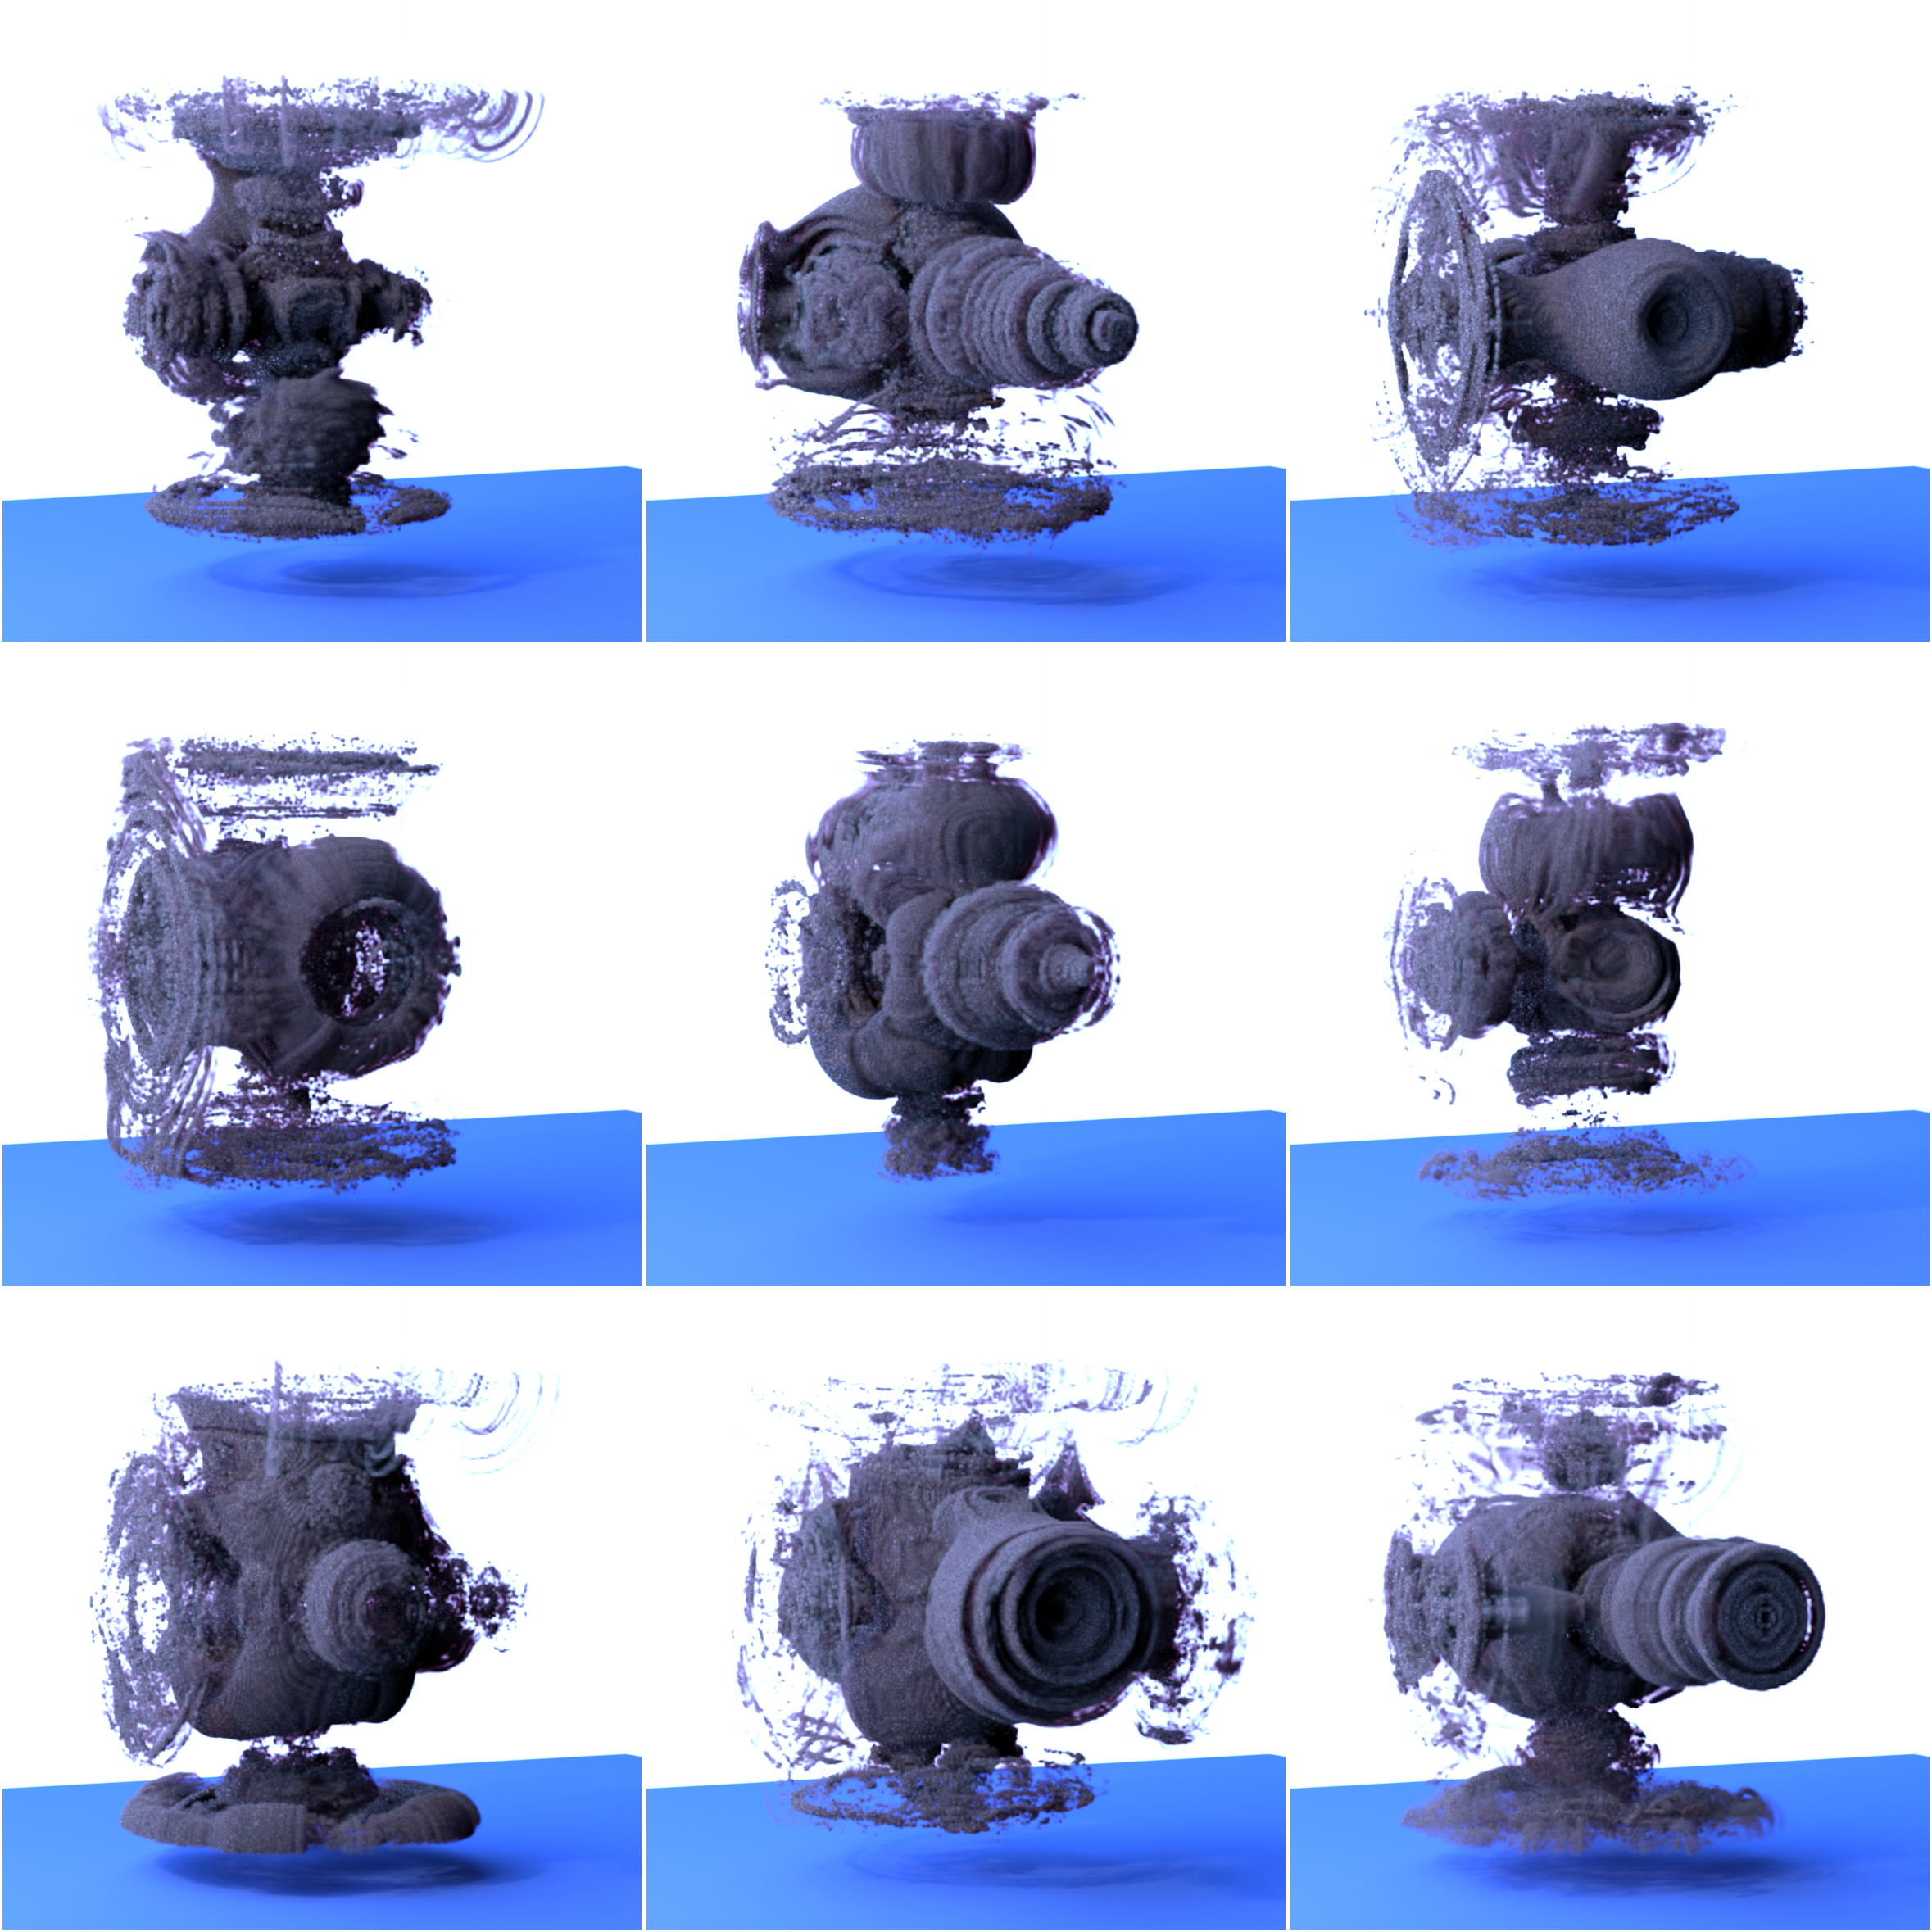
\includegraphics[width=\textwidth]{Figures/modes/montage_recolored.png}
	\caption{\em From left to right; top to bottom: An assortment of $9$ of the $150$ empirical eigenvectors, from lowest singular value to highest,  discovered by taking the combined SVD of six separate Navier-Stokes simulations. Each simulation comprises a plume of smoke moving toward a different face of the bounding box.}
	\label{fig:eigs}
\end{figure*}

%%%%%%%%%%%%%%%%%%%%%%%%%%%%%%%%%%%%%%%%%%%
Other excitation strategies are also possible, including ones that are more closely guided by the physics that generated the original input data. We can gradually activate each eigenvector in sequence and then push the resulting vector $\qq$ through existing subspace simulation algorithms which have automatically constructed approximate versions of the Navier-Stokes equations \cite{Kim2013}. Less physical approaches are also possible by treating $\qq$ as a set of mixing weights. We can then construct arbitrary paths $\varphi$, sampled at $T$ time steps $\varphi_1, \ldots, \varphi_T$, that determine the corresponding $T$ time steps of a full-coordinate velocity field. In this vein, we show the fluid simulation that results from a random walk over an higher-dimensional sphere of constant radius in the supplemental video. 

%%%%%%%%%%%%%%%%%%%%%%%%%%%%%%%%%%%%%%%%%%%
\section*{Sonification}

\begin{figure*}
	\begin{subfigure}[h]{0.5\textwidth}
		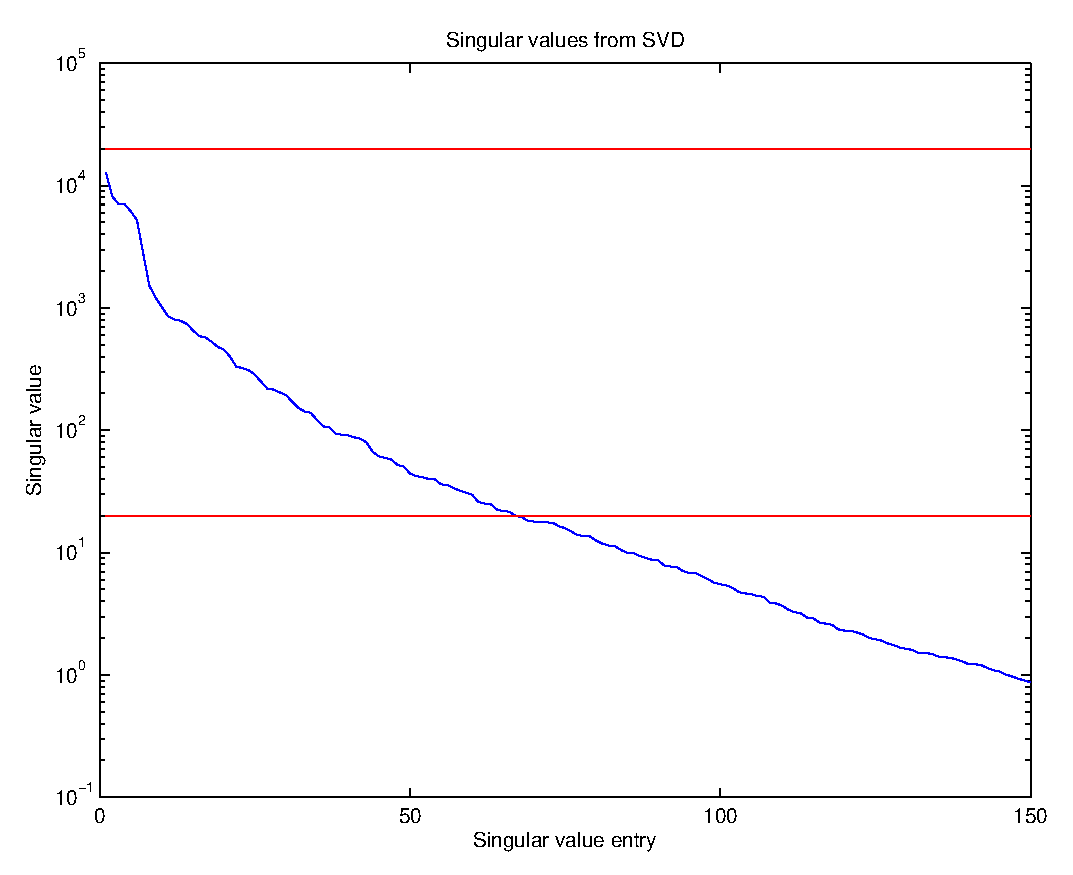
\includegraphics[width=\textwidth]{figures/singulars.eps}
		\caption{Singular values: $r$ = 150} 
		\label{fig:singulars}
	\end{subfigure}
	%
	\begin{subfigure}[h]{0.5\textwidth}
		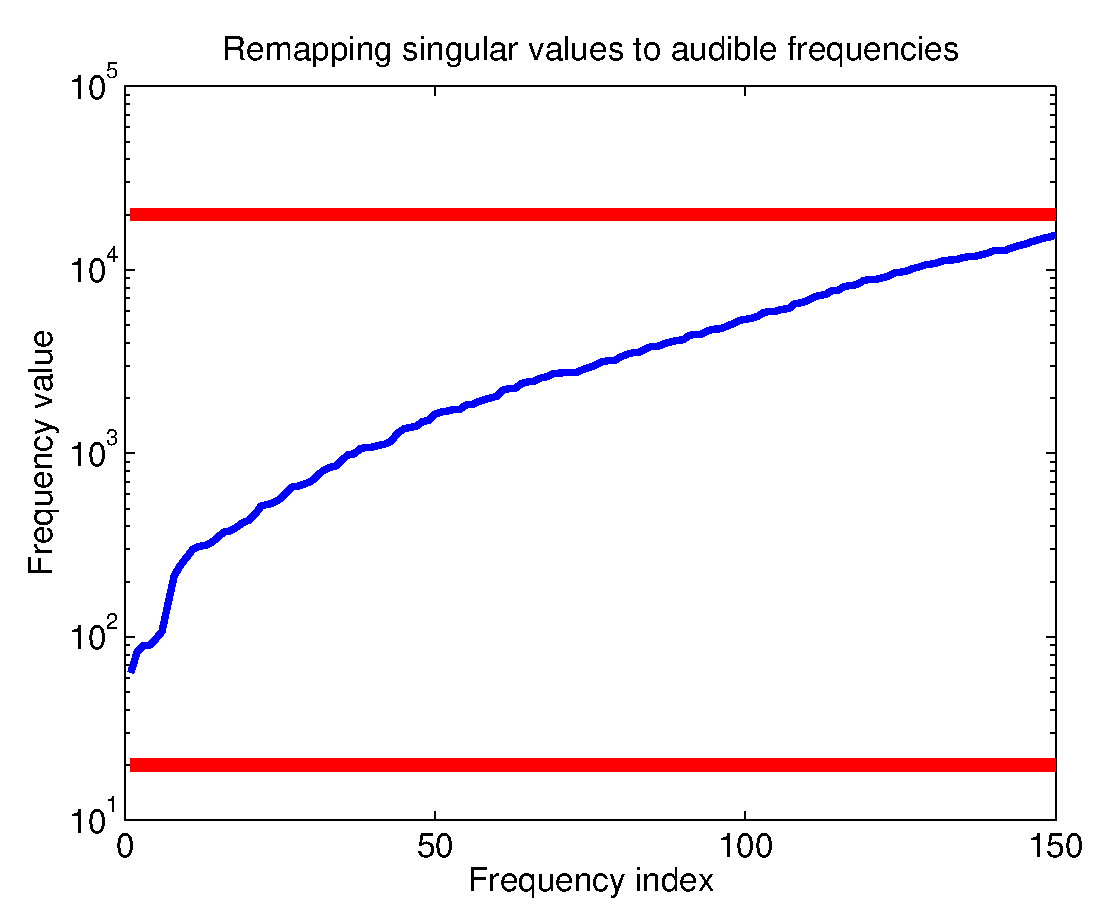
\includegraphics[width=\textwidth]{figures/remap_freqs.eps}
		\caption{Remapped frequencies: $f$ = 64 Hz, $s$ = 1.75}
		\label{fig:freqs}
	\end{subfigure}
	\caption{\em Singular values and their remapped frequencies. Note the logarithmic scale on both y-axes. The red lines on both plots indicate the bounds of the human audible frequency range.}
\end{figure*}

We will devise a strategy for converting the motion of a fluid into a sound. As mentioned previously, one of the main advantages of the empirical eigenvectors approach is that it already yields a quasi-frequency spectrum. However, some additional choices need to be made before these vectors can be made audible. This sequence of subjective but judicious choices is known as sonification. More precisely, according to Hermann \cite{hermann2008}, sonification is the ``data-dependent, systematic generation of sound.''

We begin by interpreting the $r$ singular values $\sigma_1, \ldots, \sigma_r$ from the singular-value decomposition as characteristic frequencies. There are two immediate concerns about this raw data. First, we can see in Figure \ref{fig:singulars} that the values range over approximately $4$ orders of magnitude, which is approximately $13$ octaves, and decrease to numbers less than $1$. However, the human audible frequency range begins at $20$ Hz and spans approximately $10$ octaves, up to $20000$ Hz \cite{rosen2011signals}. Thus, we must somehow normalize the data to this audible range. Secondly, the singular value spectrum begins with a maximum value and then decreases, whereas an audio spectrum starts at fundamental frequency and then increases. Hence, we invert the singular values. One way to construct a practical mapping is to specify a fundamental frequency $f$ and octave scaling $s$. Writing our audible frequencies as $f_1, \ldots, f_r$, we can define our mapping from singular values to audible frequencies as follows:

\begin{equation} 
\begin{aligned}
f_i &= f \cdot \left(\frac{\sigma_{i}^{-1}}{\sigma_{\textnormal{max}}^{-1}}\right)^{\frac{1}{s}} \\
&= f \cdot \left(\frac{\sigma_{\textnormal{max}}}{\sigma_i}\right)^{\frac{1}{s}}, \ i = 1, \ldots, r.
\end{aligned}
\end{equation}

The effect of this remapping can be seen in Figure \ref{fig:freqs}, where we have used a fundamental frequency of $f = 64$ Hz and an octave scaling of $s = 1.75$. The spectrum now begins at the fundamental, $f = 64$ Hz, and ranges up to a maximum of approximately $15000$ Hz, which is an acoustically acceptable spread.

With an audible spectrum established, we now choose amplitudes for each individual frequency. These can be mapped from a corresponding subspace vector $\qq \in \R^r$, as each of its $r$ components, $q_1, \ldots, q_r$ can be thought of as an amplitude for the $r$ corresponding frequencies $f_1, \ldots, f_r$. Care must be taken here to ensure that sum of all the amplitudes does not exceed unity gain, as this would lead to clipping. More concretely, we constrain the $L_1$ norm of $\qq$, $\lvert\qq\rvert_1 = \sum_{i=1}^{r}\lvert q_i \rvert$, to be at most $1$. A typical subspace vector $\qq$ may also contain negative components. However, these can simply be thought of as encoding a positive amplitude and a reversal of phase. The phase reversal can be discarded, as its perceivable effect is typically undesirable clicking artifacts.

With these considerations in hand, we design a mapping from a subspace vector $\qq$ to an amplitude vector $\aaa$ of unit $L_1$ norm as follows:
\begin{equation}
\begin{aligned}
a_i &= \frac{\lvert q_i \rvert}{\lvert\qq\rvert_1}, \ i = 1, \ldots, r.
\end{aligned}
\end{equation}
Given a sequence $(\qq_t)$ of vectors that describe a sampled trajectory $\qq_1, \ldots, \qq_T$ through the subspace $\R^r$, we can normalize each $\aaa_t$ vector individually. Alternatively, we can determine which $\qq_t$ has the maximum $L_1$ norm, which we denote ${\qq}_\textnormal{max}$, and normalize based on $\lvert\qq_{\textnormal{max}}\rvert_1$. The effect of the former is a relatively uniform volume level, while the latter yields a more variable volume envelope. Each approach has its own musical merit, depending on the compositional situation.

%%%%%%%%%%%%%%%%%%%%%%%%%%%%%%%%%%%%%%%%%%%
\section*{Synthesis}

With our mappings carried out, we can now produce an audible sound. To illustrate the basic mapping between the visual forms of the eigenvectors and their corresponding remapped frequencies, we move sequentially through the eigenvectors and their corresponding frequencies in the first supplemental video \cite{sequential}.This mapping generates a musical scale, and compositional operations can be carried out at the note level. For example, by scrambling the order of the frequencies and adding some rhythmic variety, we can produce a short melody, as demonstrated in the second supplemental video \cite{melody}.

% ADJ: Here is the code to generate the footnote citations of the YouTube URLs instead:
% {\tt sequential}\footnote{\url{https://youtu.be/cB79S4NwCHc}}
% {\tt melody}\footnote{\url{https://youtu.be/N6fzJXbn2ts}} 

The previous example essentially capture freeze frames of each individual mode. However, a smoother, more sophisticated auditory mapping is needed if we want to capture the flow of the smoke through mixtures of the modes. As a point of departure, we use subtractive synthesis, which passes a spectrally rich input signal through various filters in order to alter its timbre. In our case, we construct a filter bank that attenuates the input signal everywhere except at the resonant frequencies that correspond to the active modes. A particular amplitude vector $\aaa$ with component $a_i$ then tells us the strength with which each corresponding frequency $f_i$ will resonate. The nature of the input sound also strongly influences the resulting timbre; noise creates a more atmospheric effect, while impulses can create driving rhythmic textures. To match the fluid feel of the smoke propagation, we use broadband noise for the primary sound examples in this paper.

%%%%%%%%%%%%%%%%%%%%%%%%%%%%%%%%%%%%%%%%%%%
\section*{Time Evolution}
Static sound, while interesting as a new timbre for a few seconds, eventually grows stale. Thus, we would like to capture the time evolution of the subspace trajectory as a dynamic sonic event. This can be achieved by cycling through the the sequence of amplitude vectors $\aaa_1, \ldots, \aaa_T$ corresponding to the subspace trajectory $\qq_1, \ldots, \qq_T$. Using subtractive synthesis, as described above, we can generate a corresponding sound signal that changes subtly at each time step $t$. As previously discussed, different trajectories through the subspace generate different sequences of amplitude vectors. Musically, the unfolding of these trajectories over time occurs on a micro-scale, but the overall effect is perceived smoothly, much as the individual frames of a video fuse together into a continuous motion.

Experimentally, we have explored several different categories of subspace trajectories. In the third supplemental video \cite{reduced}, we gradually activate each eigenvector in sequence and push the resulting subspace vector through the reduced-space Navier-Stokes equations. In the final supplemental video {\cite{sphere}, we put aside the equations of fluid flow and walk the subspace vector $\qq$ across the surface of a sphere in $\R^r$. 

% ADJ: Here is the code to generate the footnote citations of the YouTube URLs instead:
% {\tt reduced}\footnote{\url{https://youtu.be/_DXRQZYLcdE}}
% {\tt sphere}\footnote{\url{https://youtu.be/y6zraBpH5PA}}

\section*{Conclusion}

We have performed a preliminary exploration into the visual and sonic patterns that arise from a generalized form of the Chladni plate experiment. Instead of studying the eigenvectors of the Bi-Laplacian operator, we computed the empirical eigenvectors associated with fluid flow. The resulting forms are visually striking, and the corresponding spectrum can be sonified to produce a promising compositional palette. Suspending the underlying physics and performing an abstract subspace traversal produces intriguing results, which suggest many possible avenues for future work. Indeed, the interplay between the audio and the visual forms seems to form a language that we intend to explore and codify.

%%%%%%%%%%%%%%%%%%%%%%%%%%%%%%%%%%%%%%%%%%%
%%%%%%%%%%%%%%%%%%%%%%%%%%%%%%%%%%%%%%%%%%%

% If you are only going to use a BibTeX database, from which all your cites will be
% taken and formatted consistently, use the following.

\bibliographystyle{plain}
\fontsize{10}{12}
\bibliography{mybib}

\end{document}
